% !TeX root = ../main.tex
% Add the above to each chapter to make compiling the PDF easier in some editors.

\chapter{Methods and Results}\label{chapter:introduction}


\section{Maximum Mean Discrepancy}
Maximum Mean Discrepancy (MMD) is a criterion which estimates the discrepancy between two distribution. MMD can be used to optimize the network such that the distribution discrepancy is reduced in a data domain-invariant feature space. The discrepancy is measured as squared distance between the distribution kernel embeddings in the reproducing kernel Hilbert space (RKHS). The distribution discrepancy across domains is measured in the layers of the neural network in order to avoid feature transferability degradation. One has to pay attention to not transfer noise or irrelevant information. This destroys the structure of the source and target domain data and therefore makes the classification task even more difficult \cite{li2020domain}. 

\begin{align}
    M_{k}(P,Q) = \Bigl|  \boldsymbol{E_{P}}[\Phi(\boldsymbol{X^{s}})] - \boldsymbol{E_{Q}}[\Phi(\boldsymbol{X^{t}})]     \Bigl|^{2}_{Hk}
\end{align}

Hk denotes the RKHS, which is described by the characteristic kernel k and the mapping function $\Phi$. Taking the identity function as mapping function results in matching the distribution means. When using more complex mapping functions also higher order moments can be matched \cite{Yujia2015}. The distributions of the source domain $X^{s} = \{{x}_{i}^{s}\}_{i=0,...,n_{s}}$ and target domain $X^{t} = \{{x}_{i}^{t}\}_{i=0,...,n_{t}}$ are represented by P and Q. $\boldsymbol{E_{p}[.]}$ is the expected value of the source distribution P in the feature space. The kernel choice is of great importance when applying MMD. For this reason it makes sense to combine several kernels in order to profit from their individual performance \cite{li2020domain}.

\begin{align}
    k(\boldsymbol{X^{s}}, \boldsymbol{X^{t}}) = \sum_{i=0}^{N_{k}} k_{\sigma_{i}}(\boldsymbol{X^{s}}, \boldsymbol{X^{t}})
\end{align}

$N_{k}$ denotes the number of kernels used in the the RKHS and $k_{\sigma_{i}}$ represents one individual RBF kernels. Also, other kernels like linear kernels could be used, but current research shows that RBF kernels usually perform best \cite{AZAMFAR2020103932}. In our attempt we used 5 RBF kernels with the bandwidth parameters 1, 2, 4, 8, 16.


\subsubsection{Sensitive balancing of Cross-Entropy and MMD loss} \label{sec:Balancing Cross-Entropy and MMD loss}

In the following section the influence of the weighting factor GAMMA on the training success is evaluated. The CNN of the model presented in fig. \ref{fig:model_feature_extraction_test} which acts as feature extractor is optimized with an SGD optimizer with learning rate of 0.01.


\begin{figure}[htpb]
  \centering
  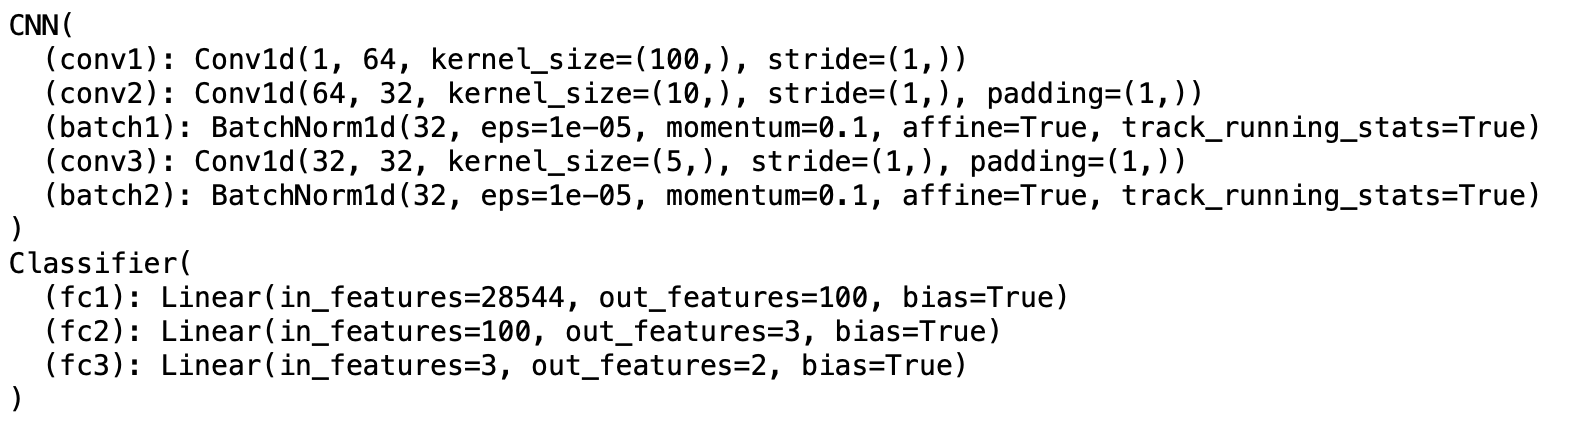
\includegraphics[width=1.1\textwidth]{model_feature_extraction_test}
  \caption {Data distribution: Influence of GAMMA to the model training with MMD loss} \label{fig:model_feature_extraction_test}
\end{figure}
\FloatBarrier 


The data distribution of the source and target domain samples in the 3D penultimate hidden layer of the classifier is visualized in fig. \ref{fig:point_cloud_mmd}. Fig. \ref{fig:learning_curves_influence_mmd_feature_extractor} shows the development of the MMD and cross entropy loss throughout the training process. When picking a small GAMMA, the model suffers from a bad separability of the two classes across the two domains. In this case the source cross-entropy loss dominates the training. Instead of reducing the domain discrepancy the model training focuses solely on predicting source samples correctly. When picking a big GAMMA the training is dominated by the MMD loss such that the correct prediction of source domain samples becomes irrelevant. Since the target labels are unknown, the MMD loss is calculated between source and target samples of the same and different classes. The MMD loss reduces the inter and intra class distance between the latent space feature vectors of source and target samples. The separability of the classes is reduced. A trivial solution for this optimization problem is a model which processes all samples such that they collapse at the same point in the latent feature space.



\begin{figure}[p]
  \centering
  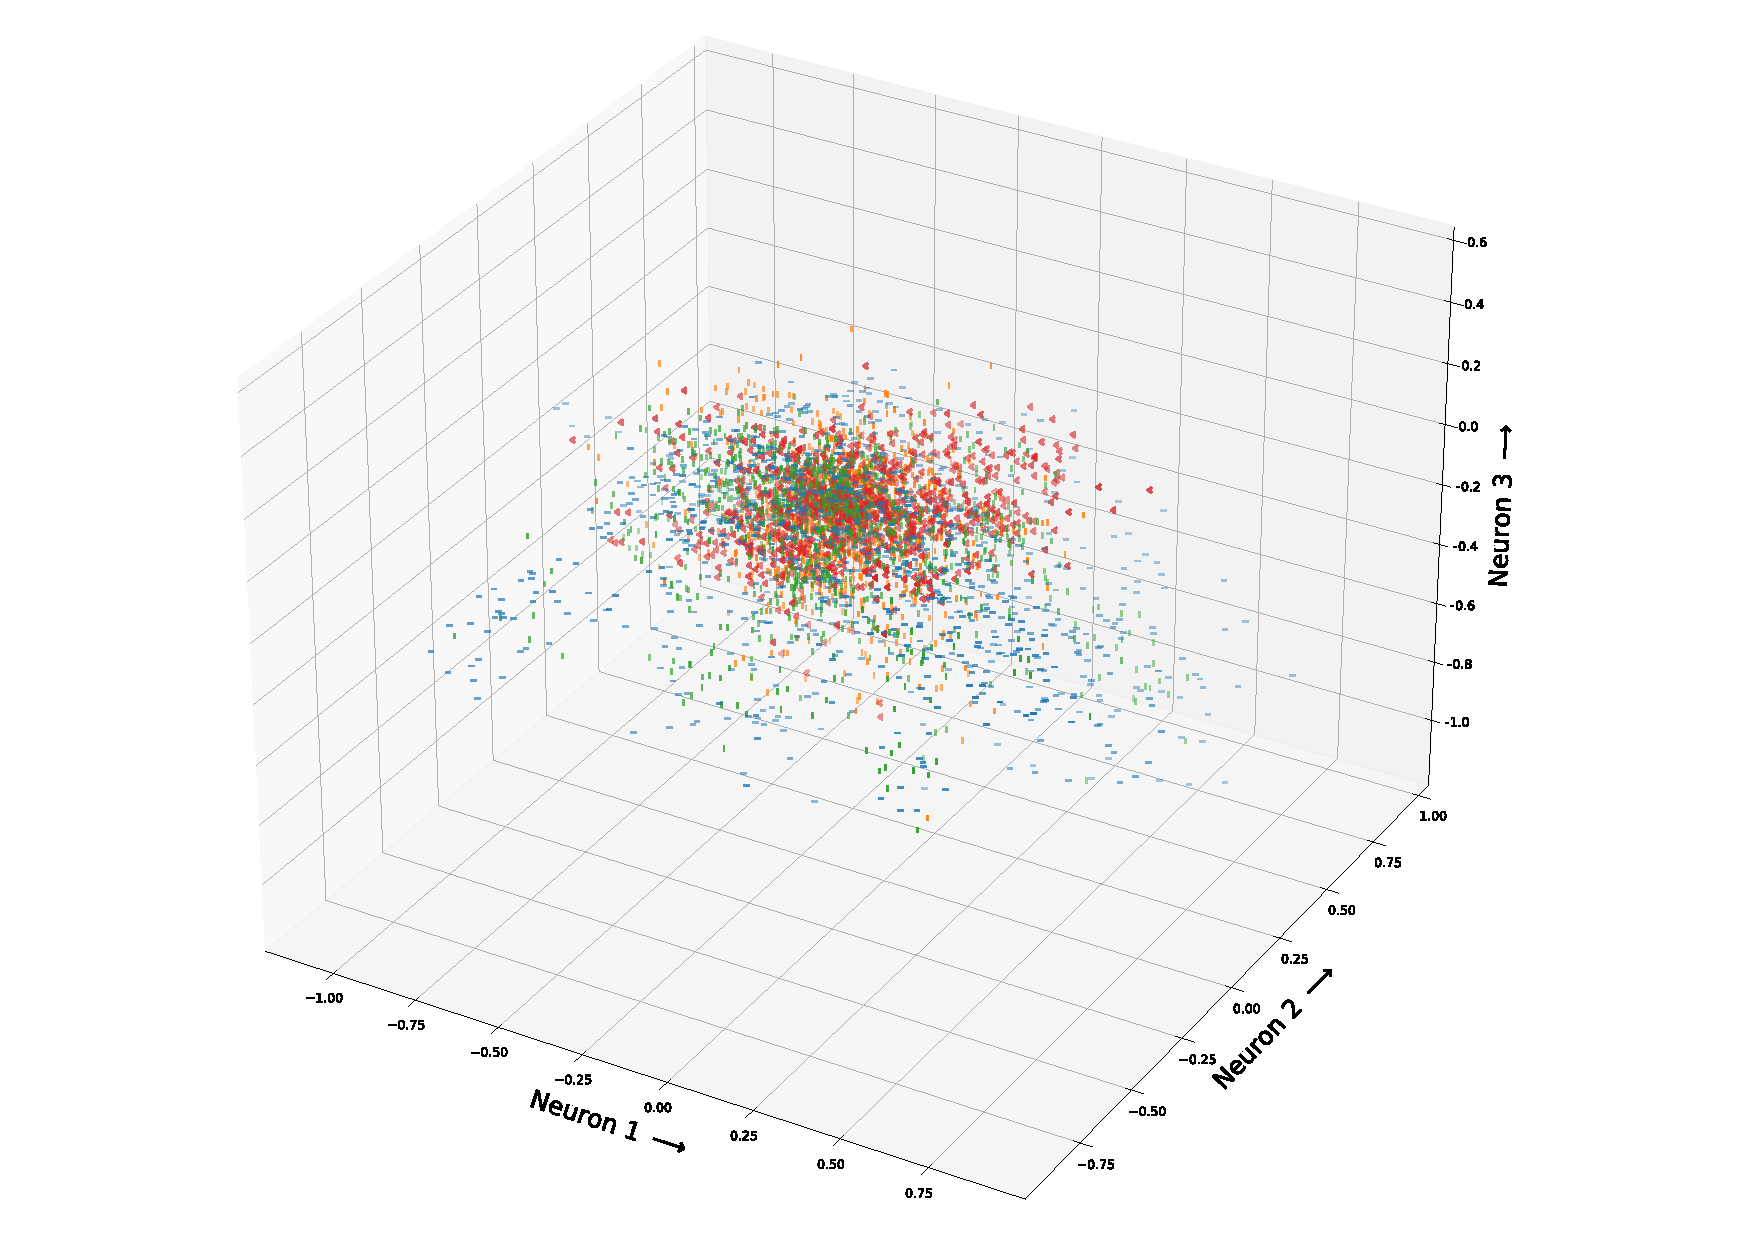
\includegraphics[width=.44\textwidth]{GAMMA_distribution/mmd_epoch0_0_1.pdf}
  \hspace{.3cm}
  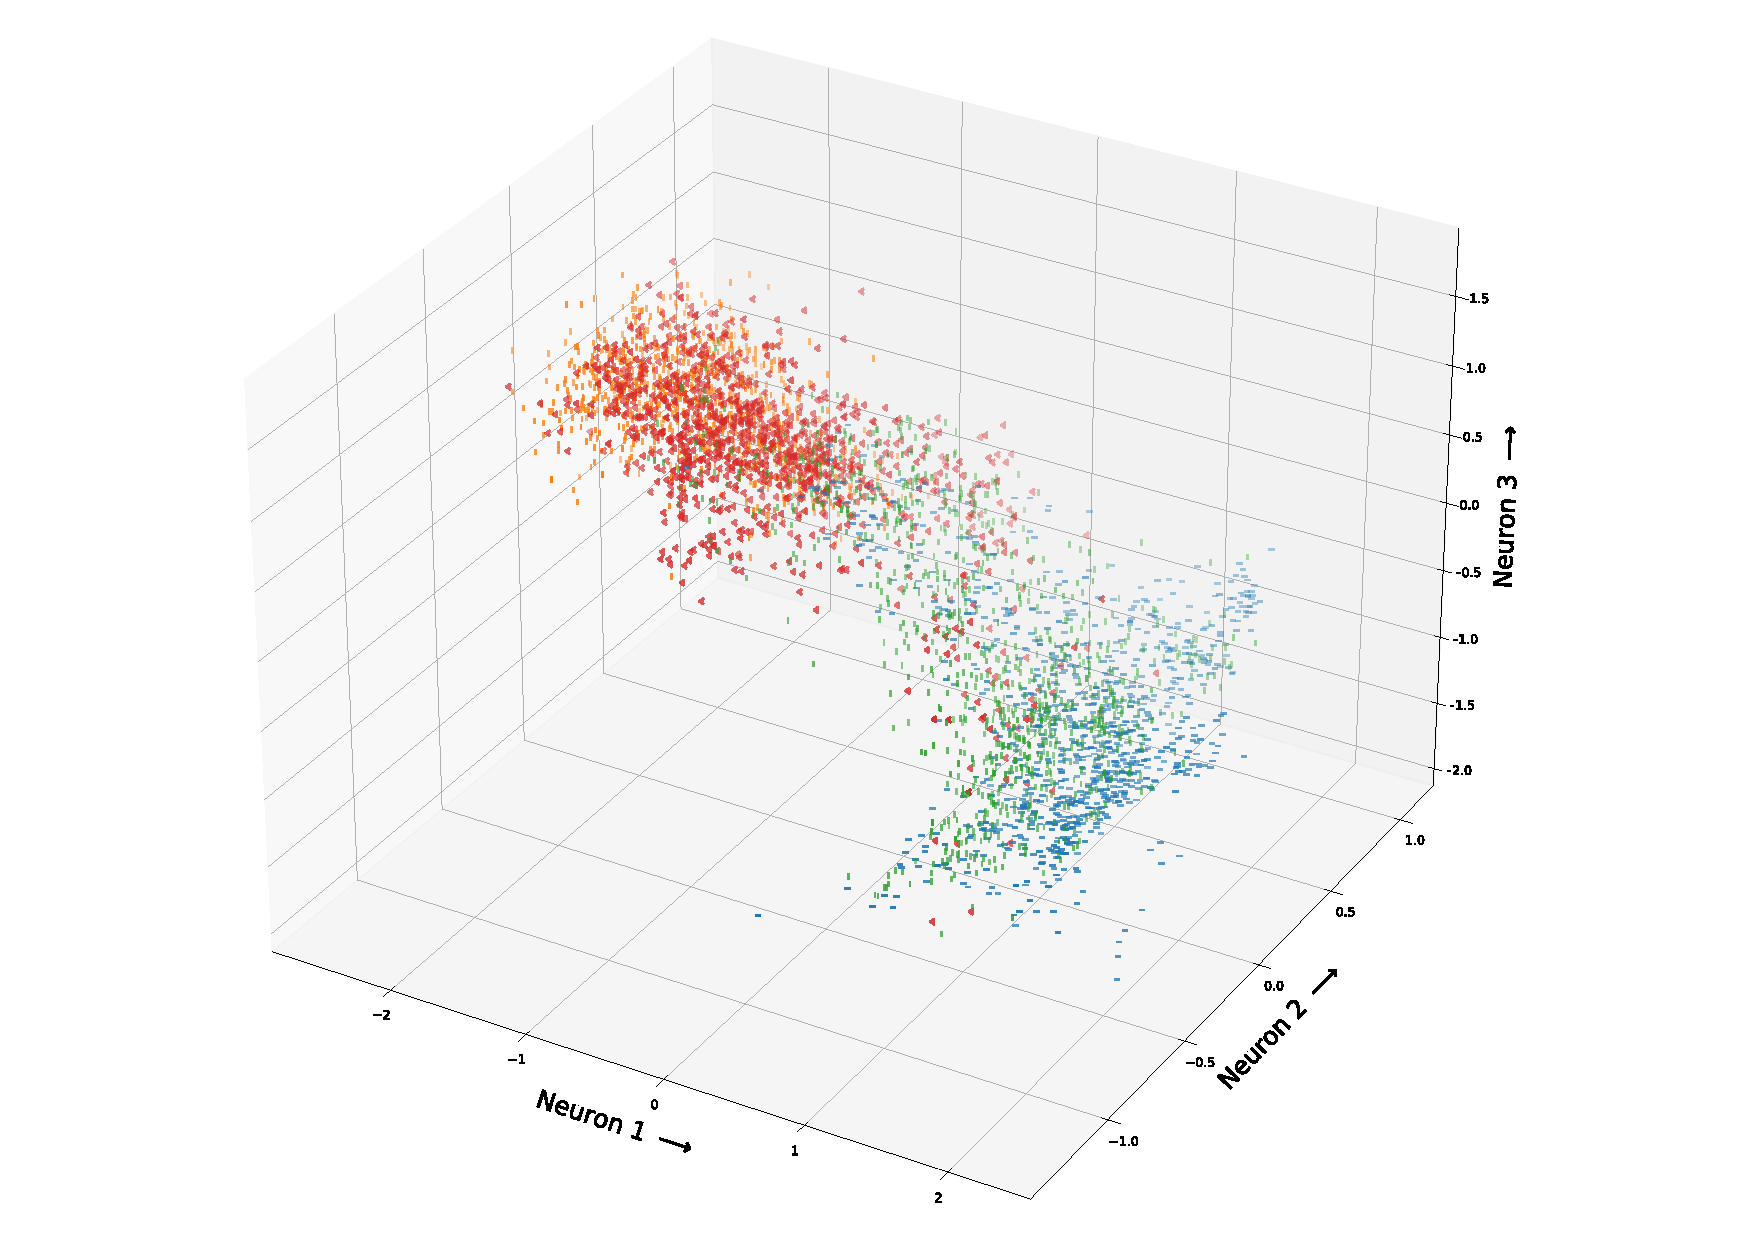
\includegraphics[width=.44\textwidth]{GAMMA_distribution/mmd_epoch8_0_1.pdf}

  \vspace{.1cm}

  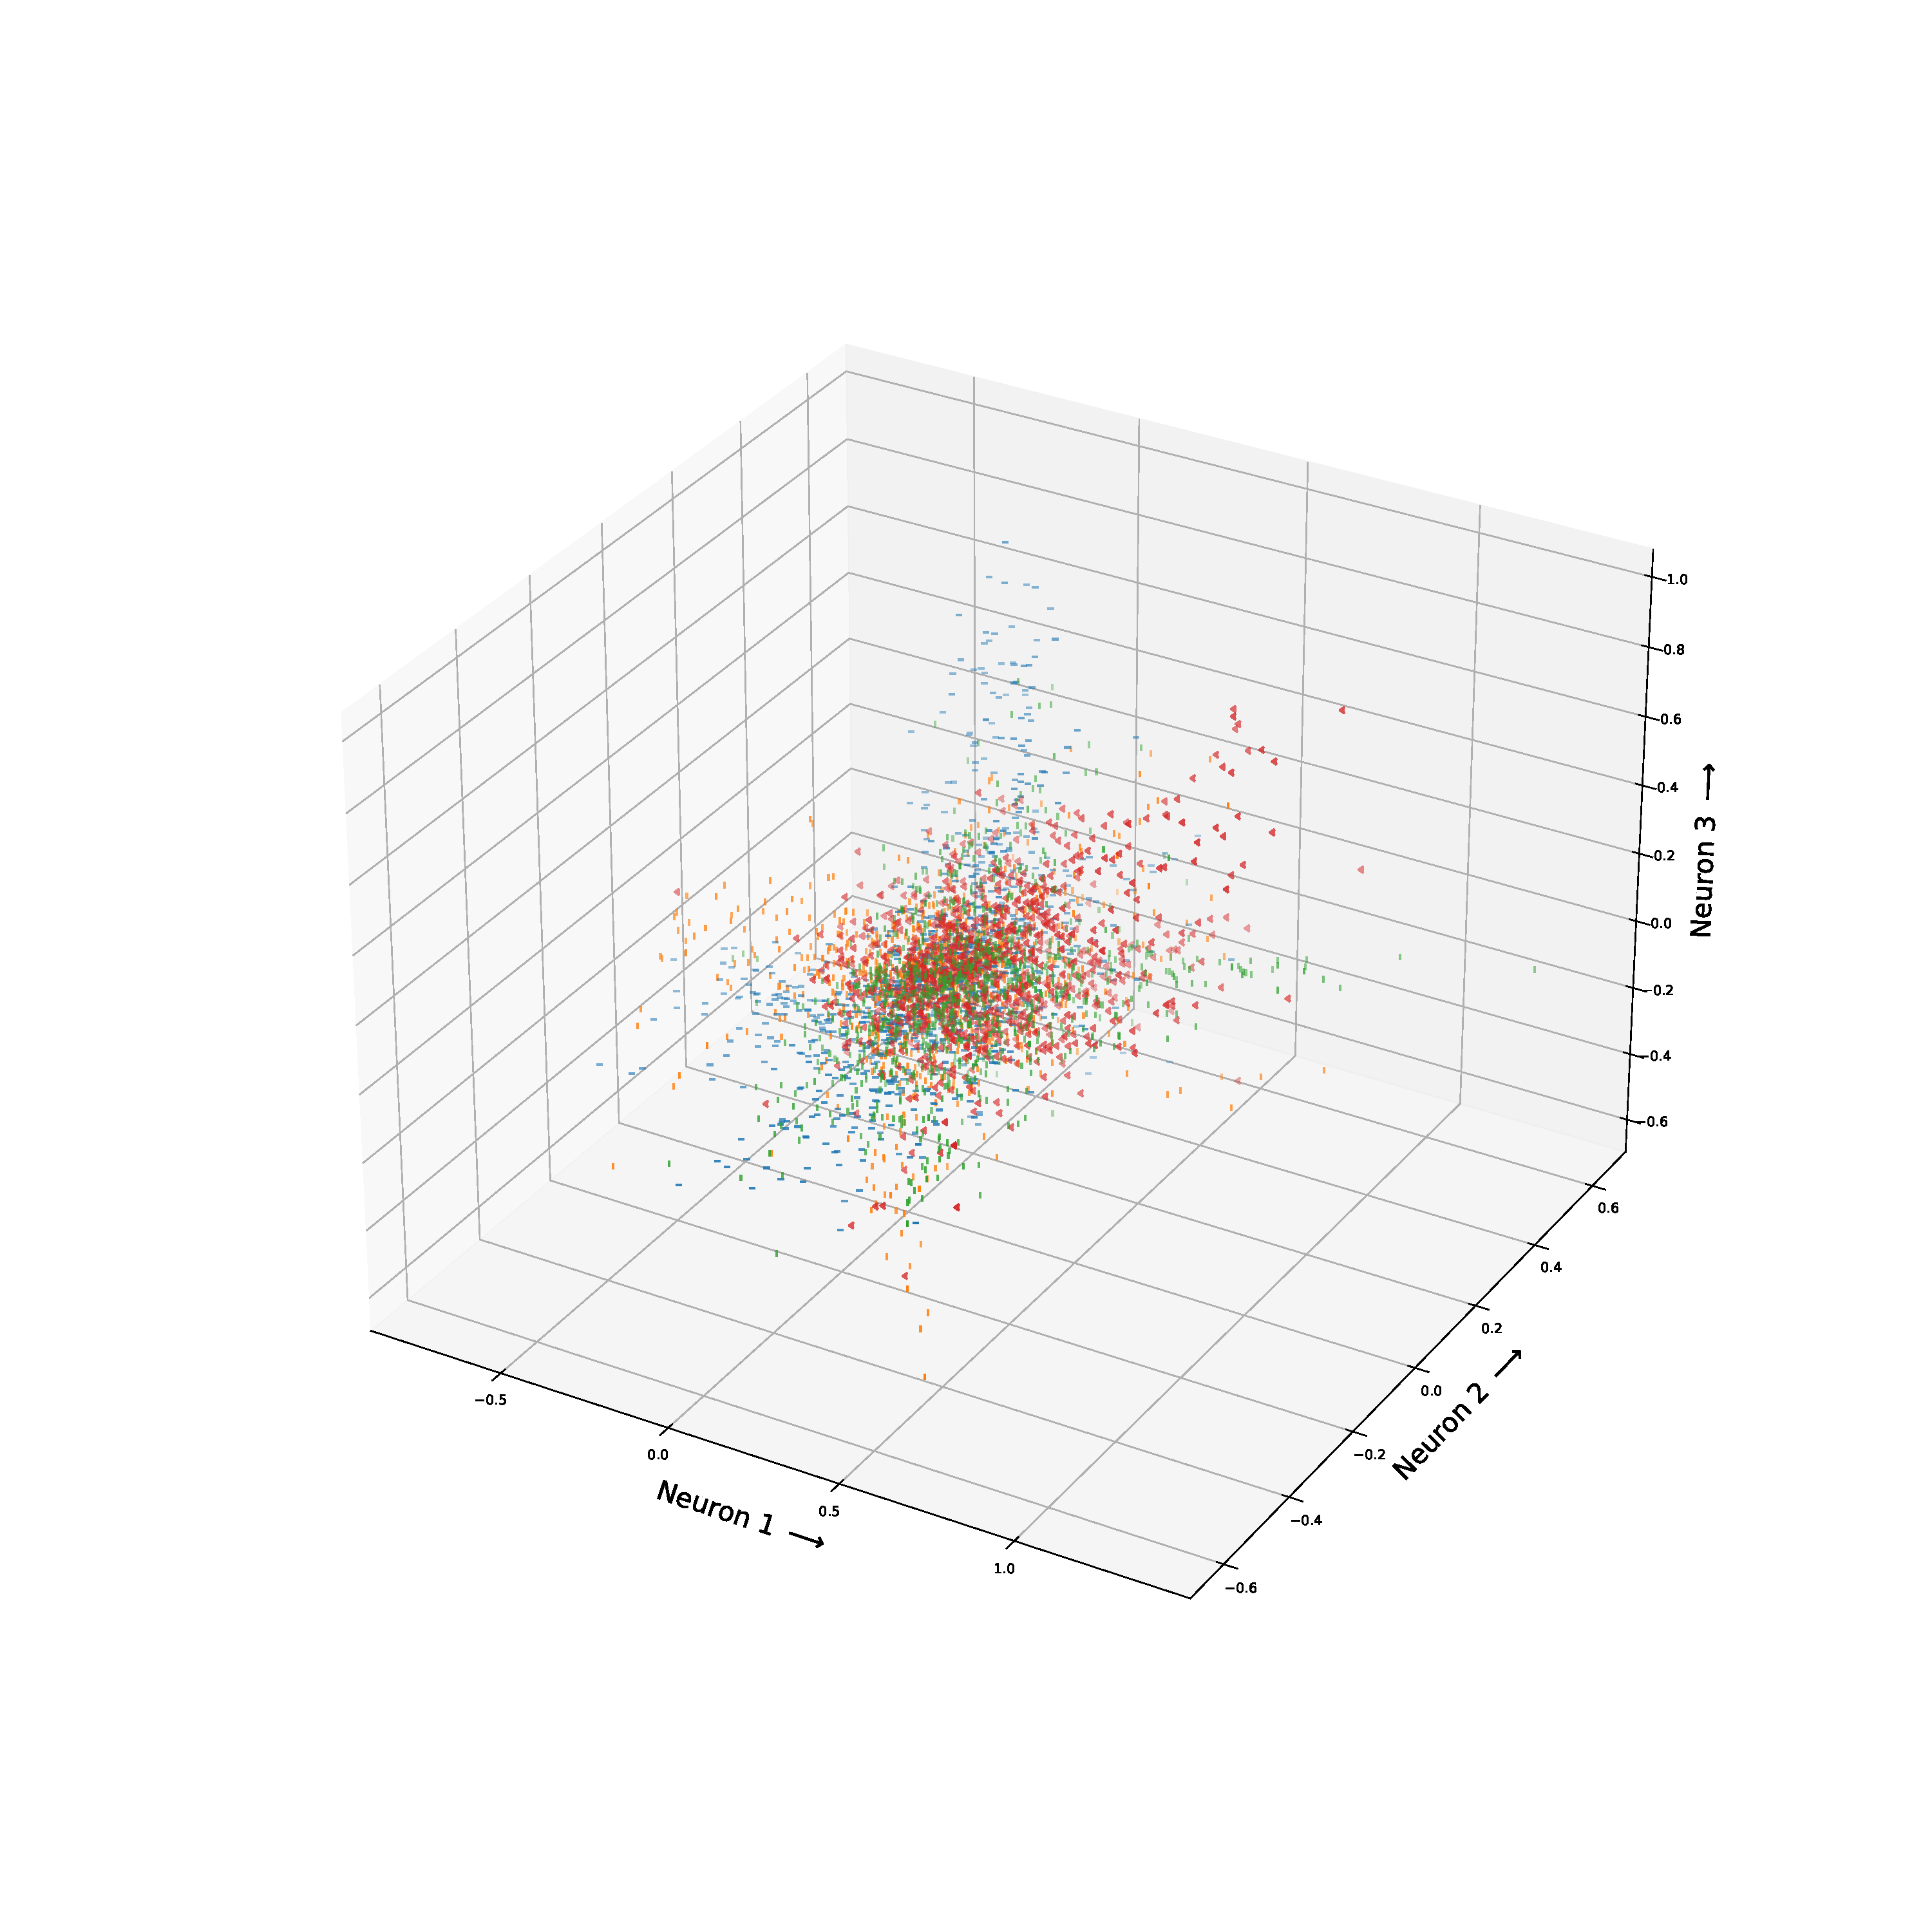
\includegraphics[width=.44\textwidth]{GAMMA_distribution/mmd_epoch0_0_5.pdf}
  \hspace{.3cm}
  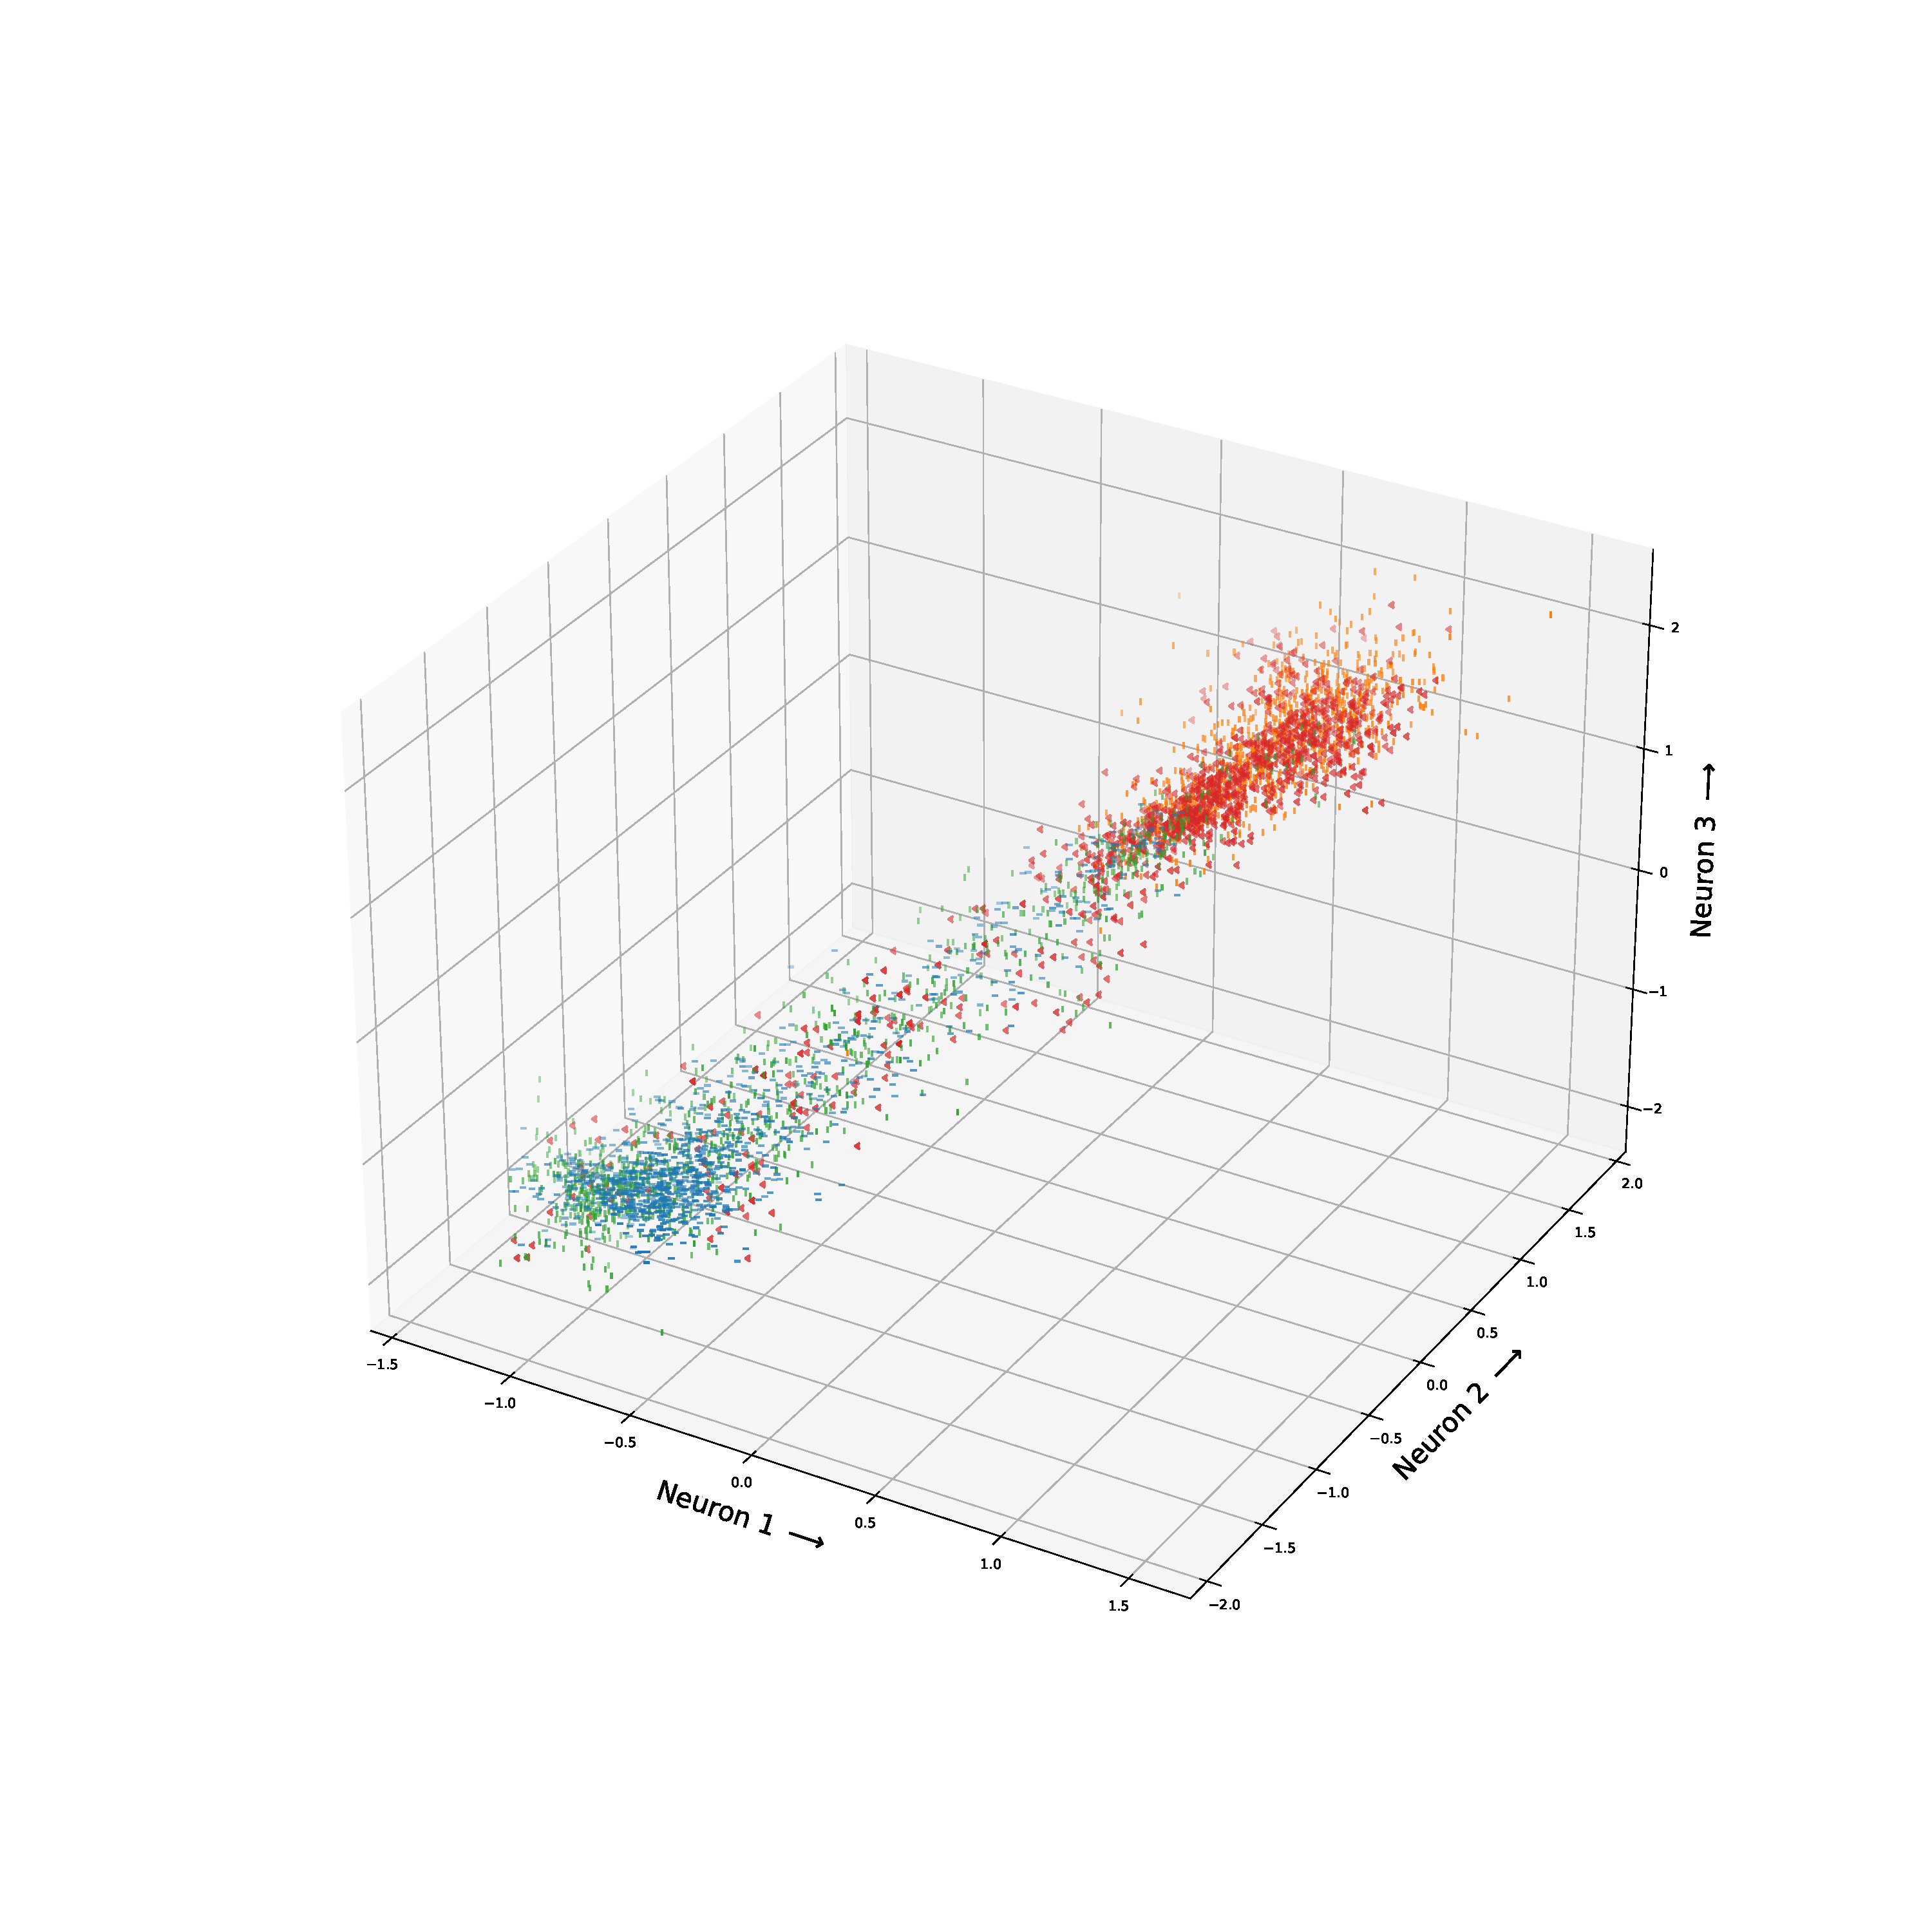
\includegraphics[width=.44\textwidth]{GAMMA_distribution/mmd_epoch8_0_5.pdf}

  \vspace{.1cm}

  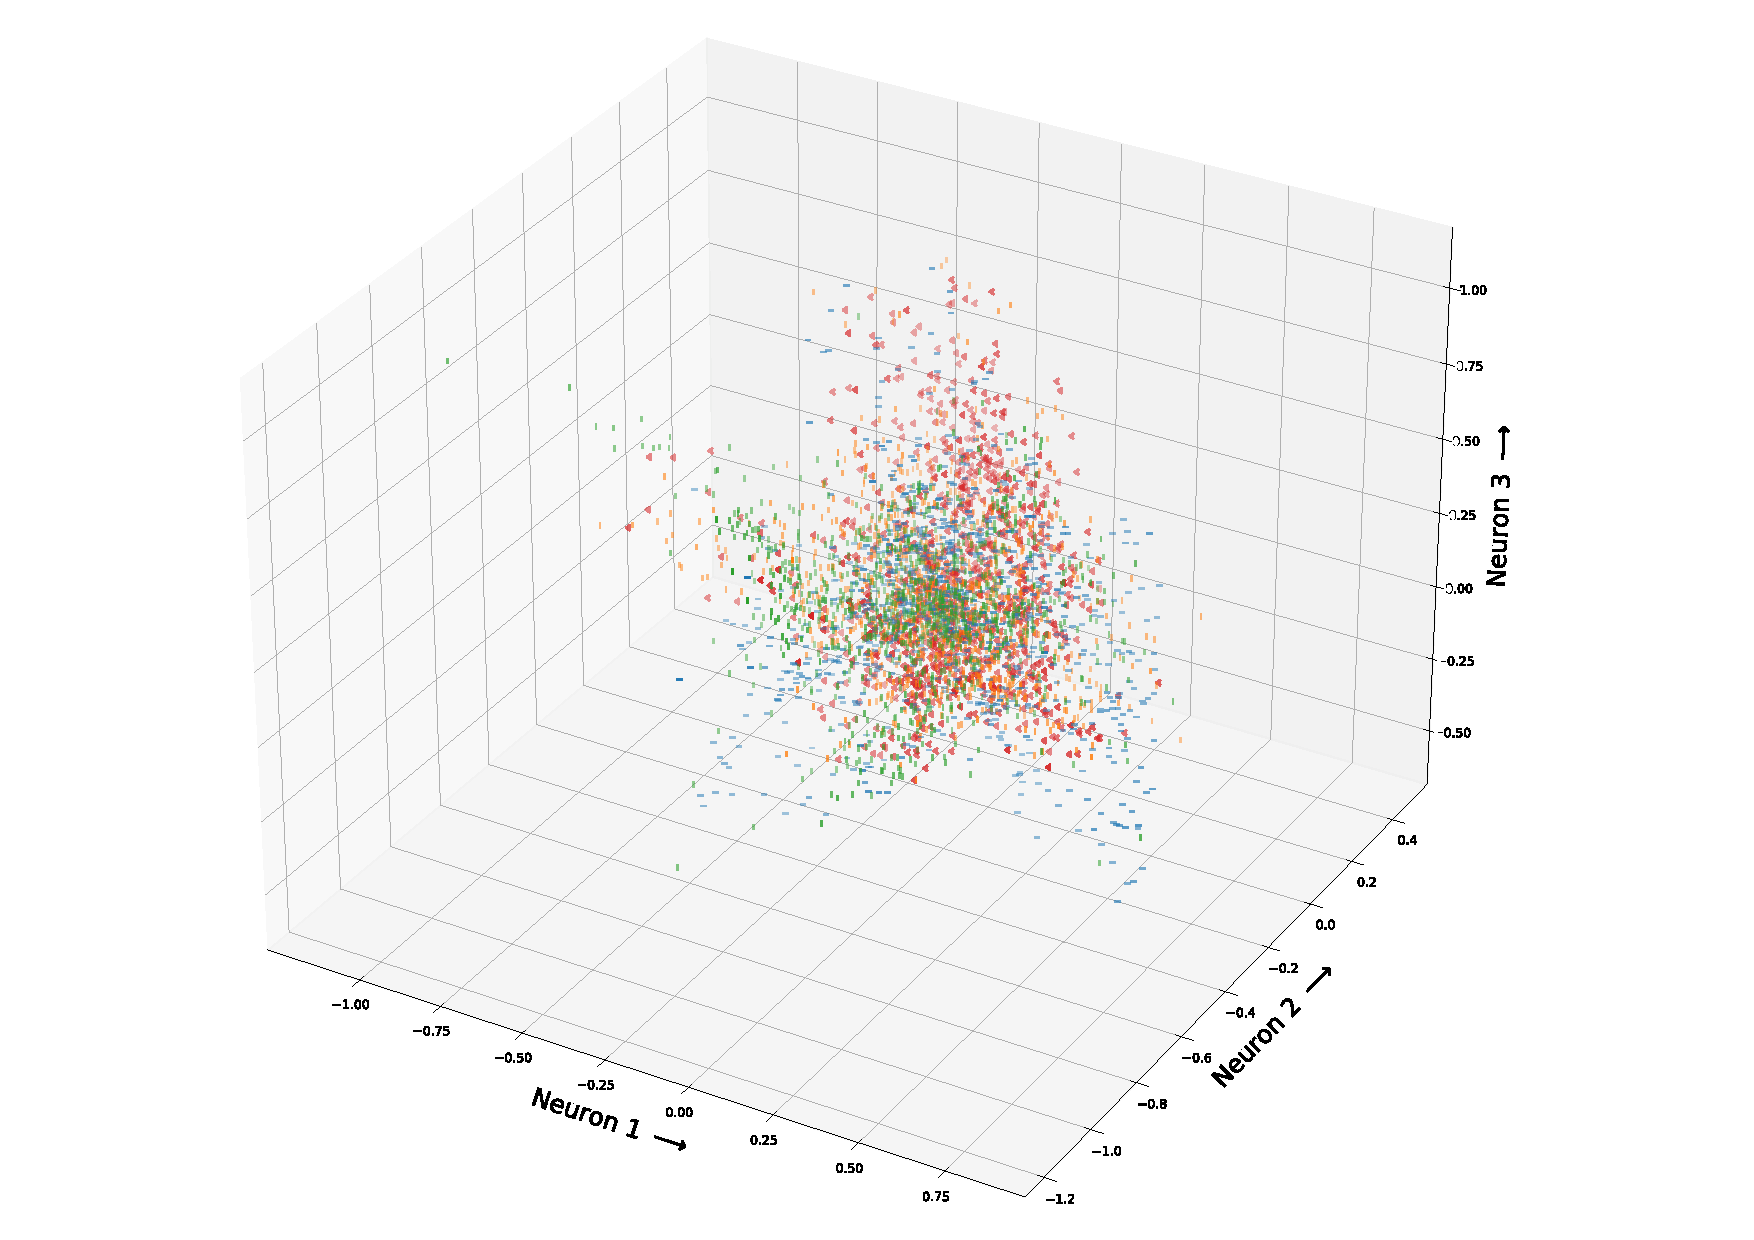
\includegraphics[width=.44\textwidth]{GAMMA_distribution/mmd_epoch0_30.pdf}
  \hspace{.3cm}
  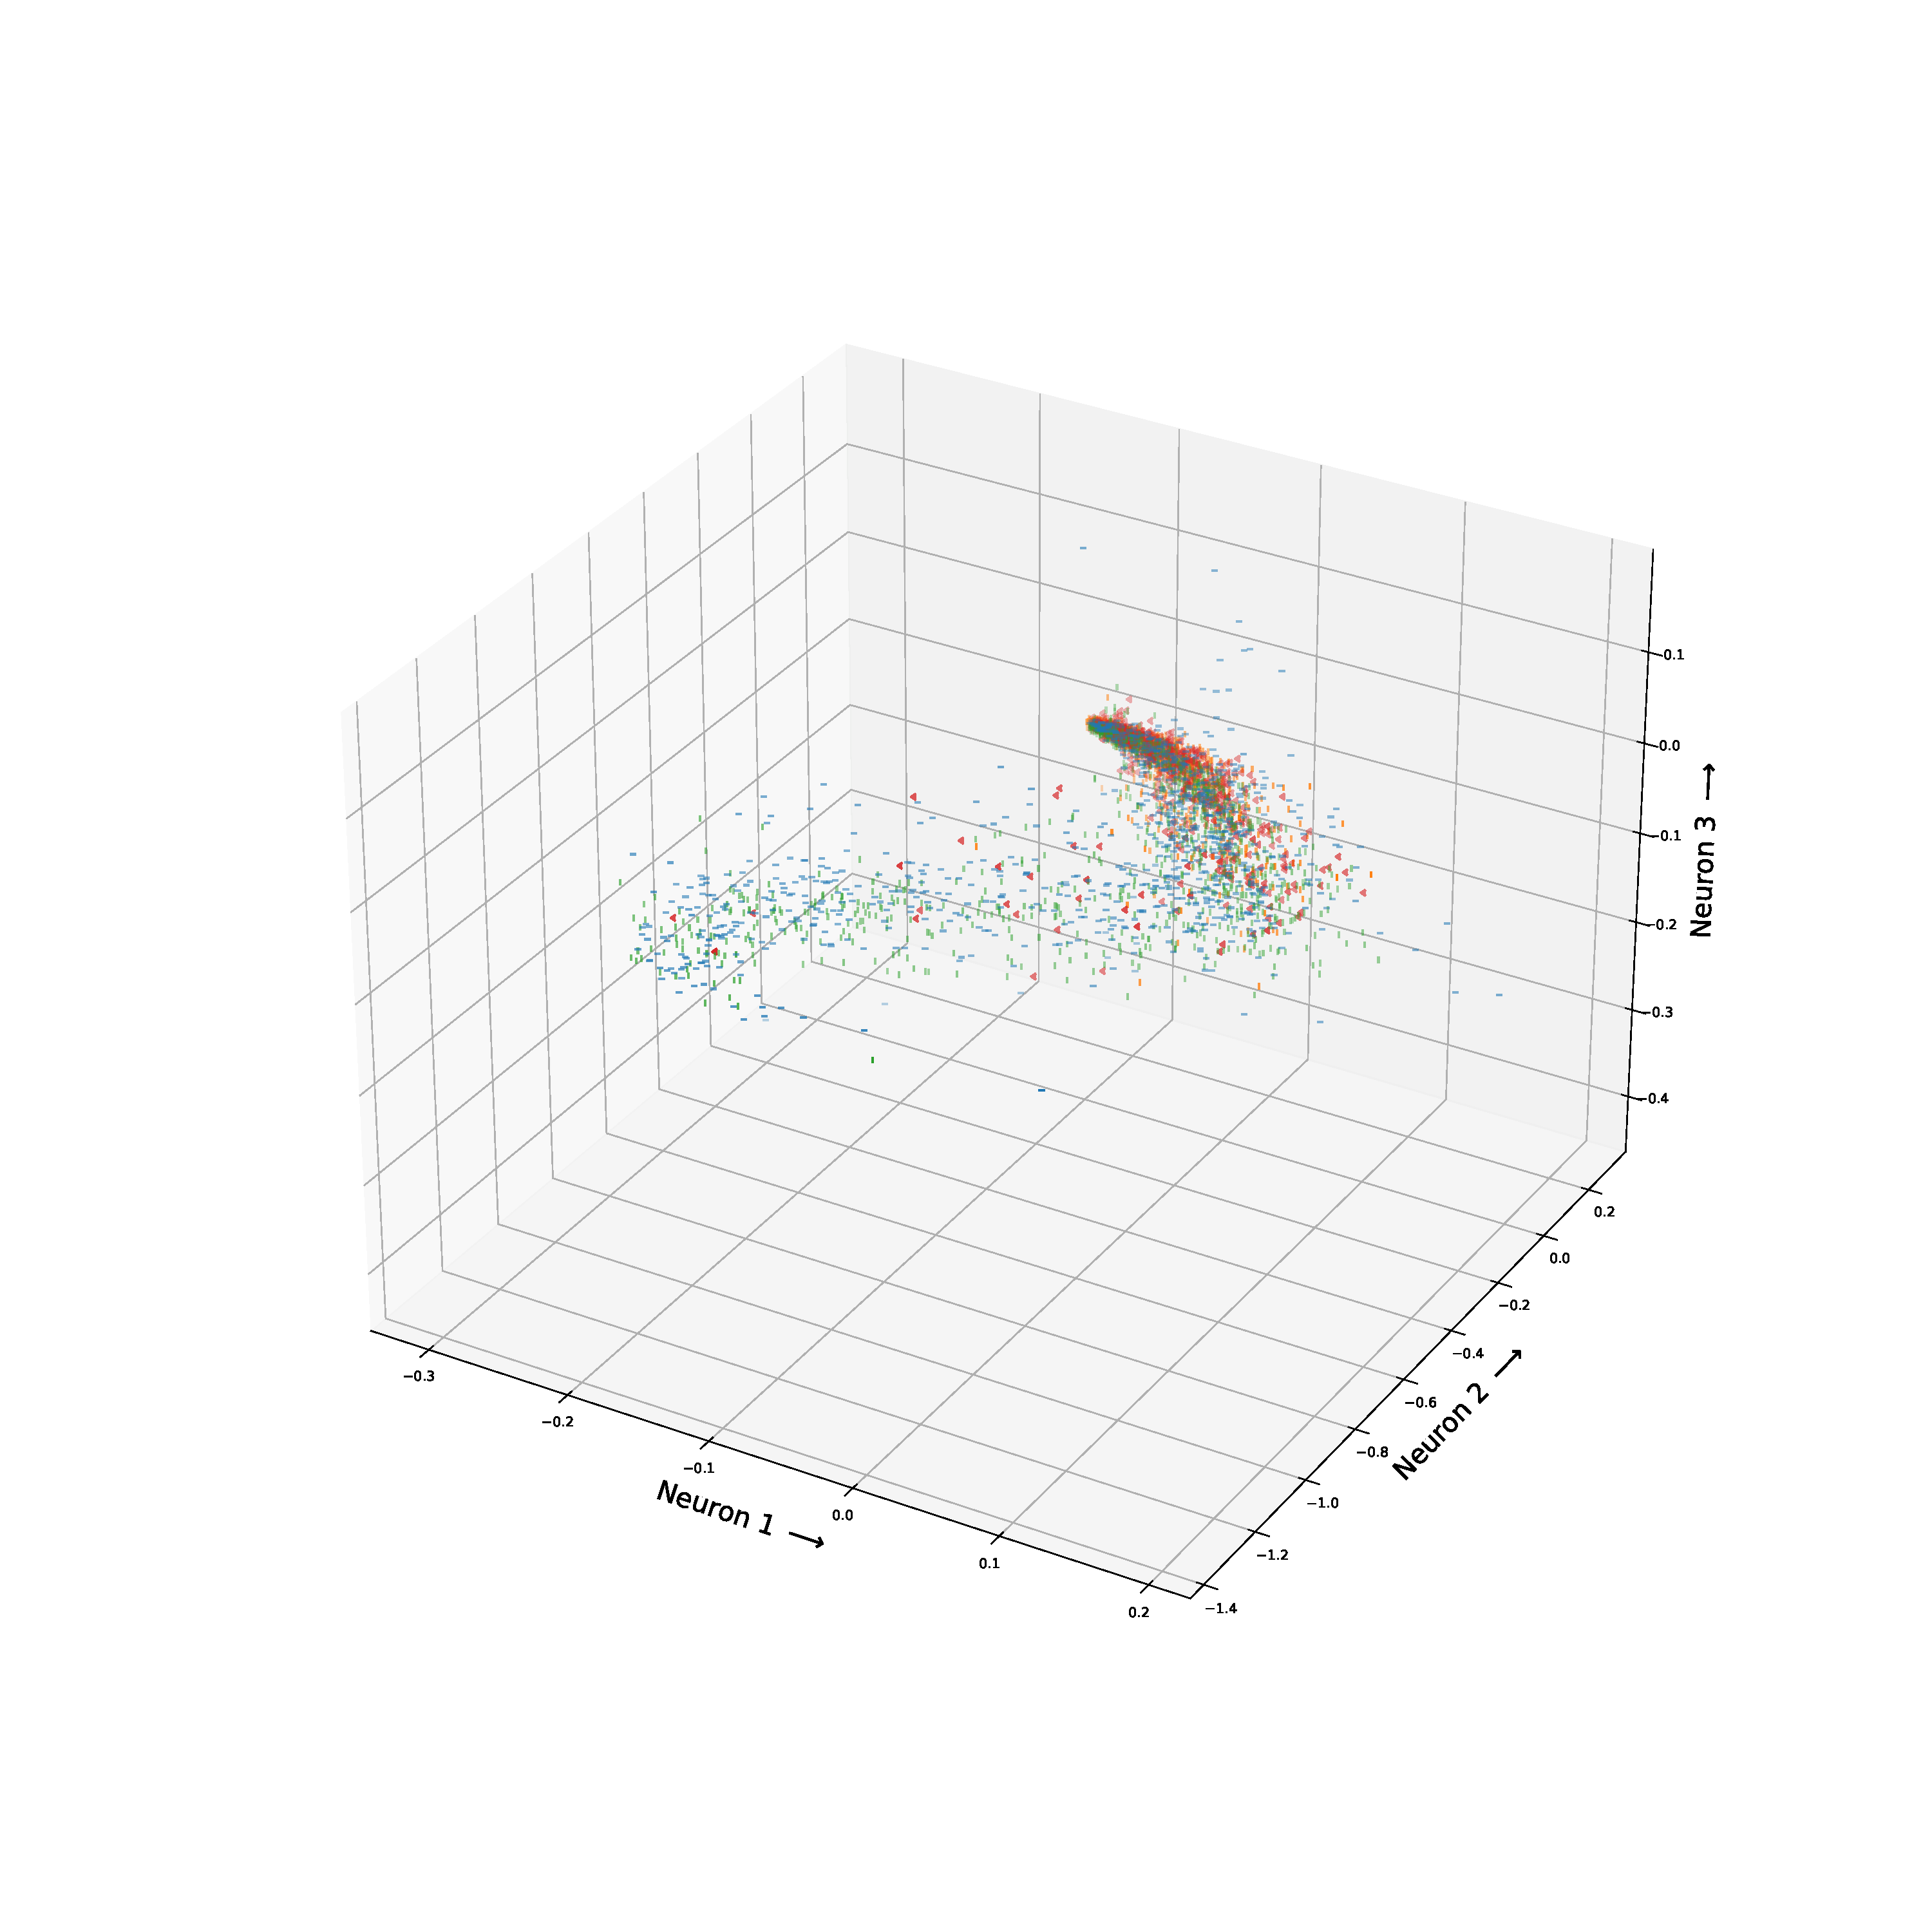
\includegraphics[width=.44\textwidth]{GAMMA_distribution/mmd_epoch8_30.pdf}
  
  \vspace{.1cm}
  
  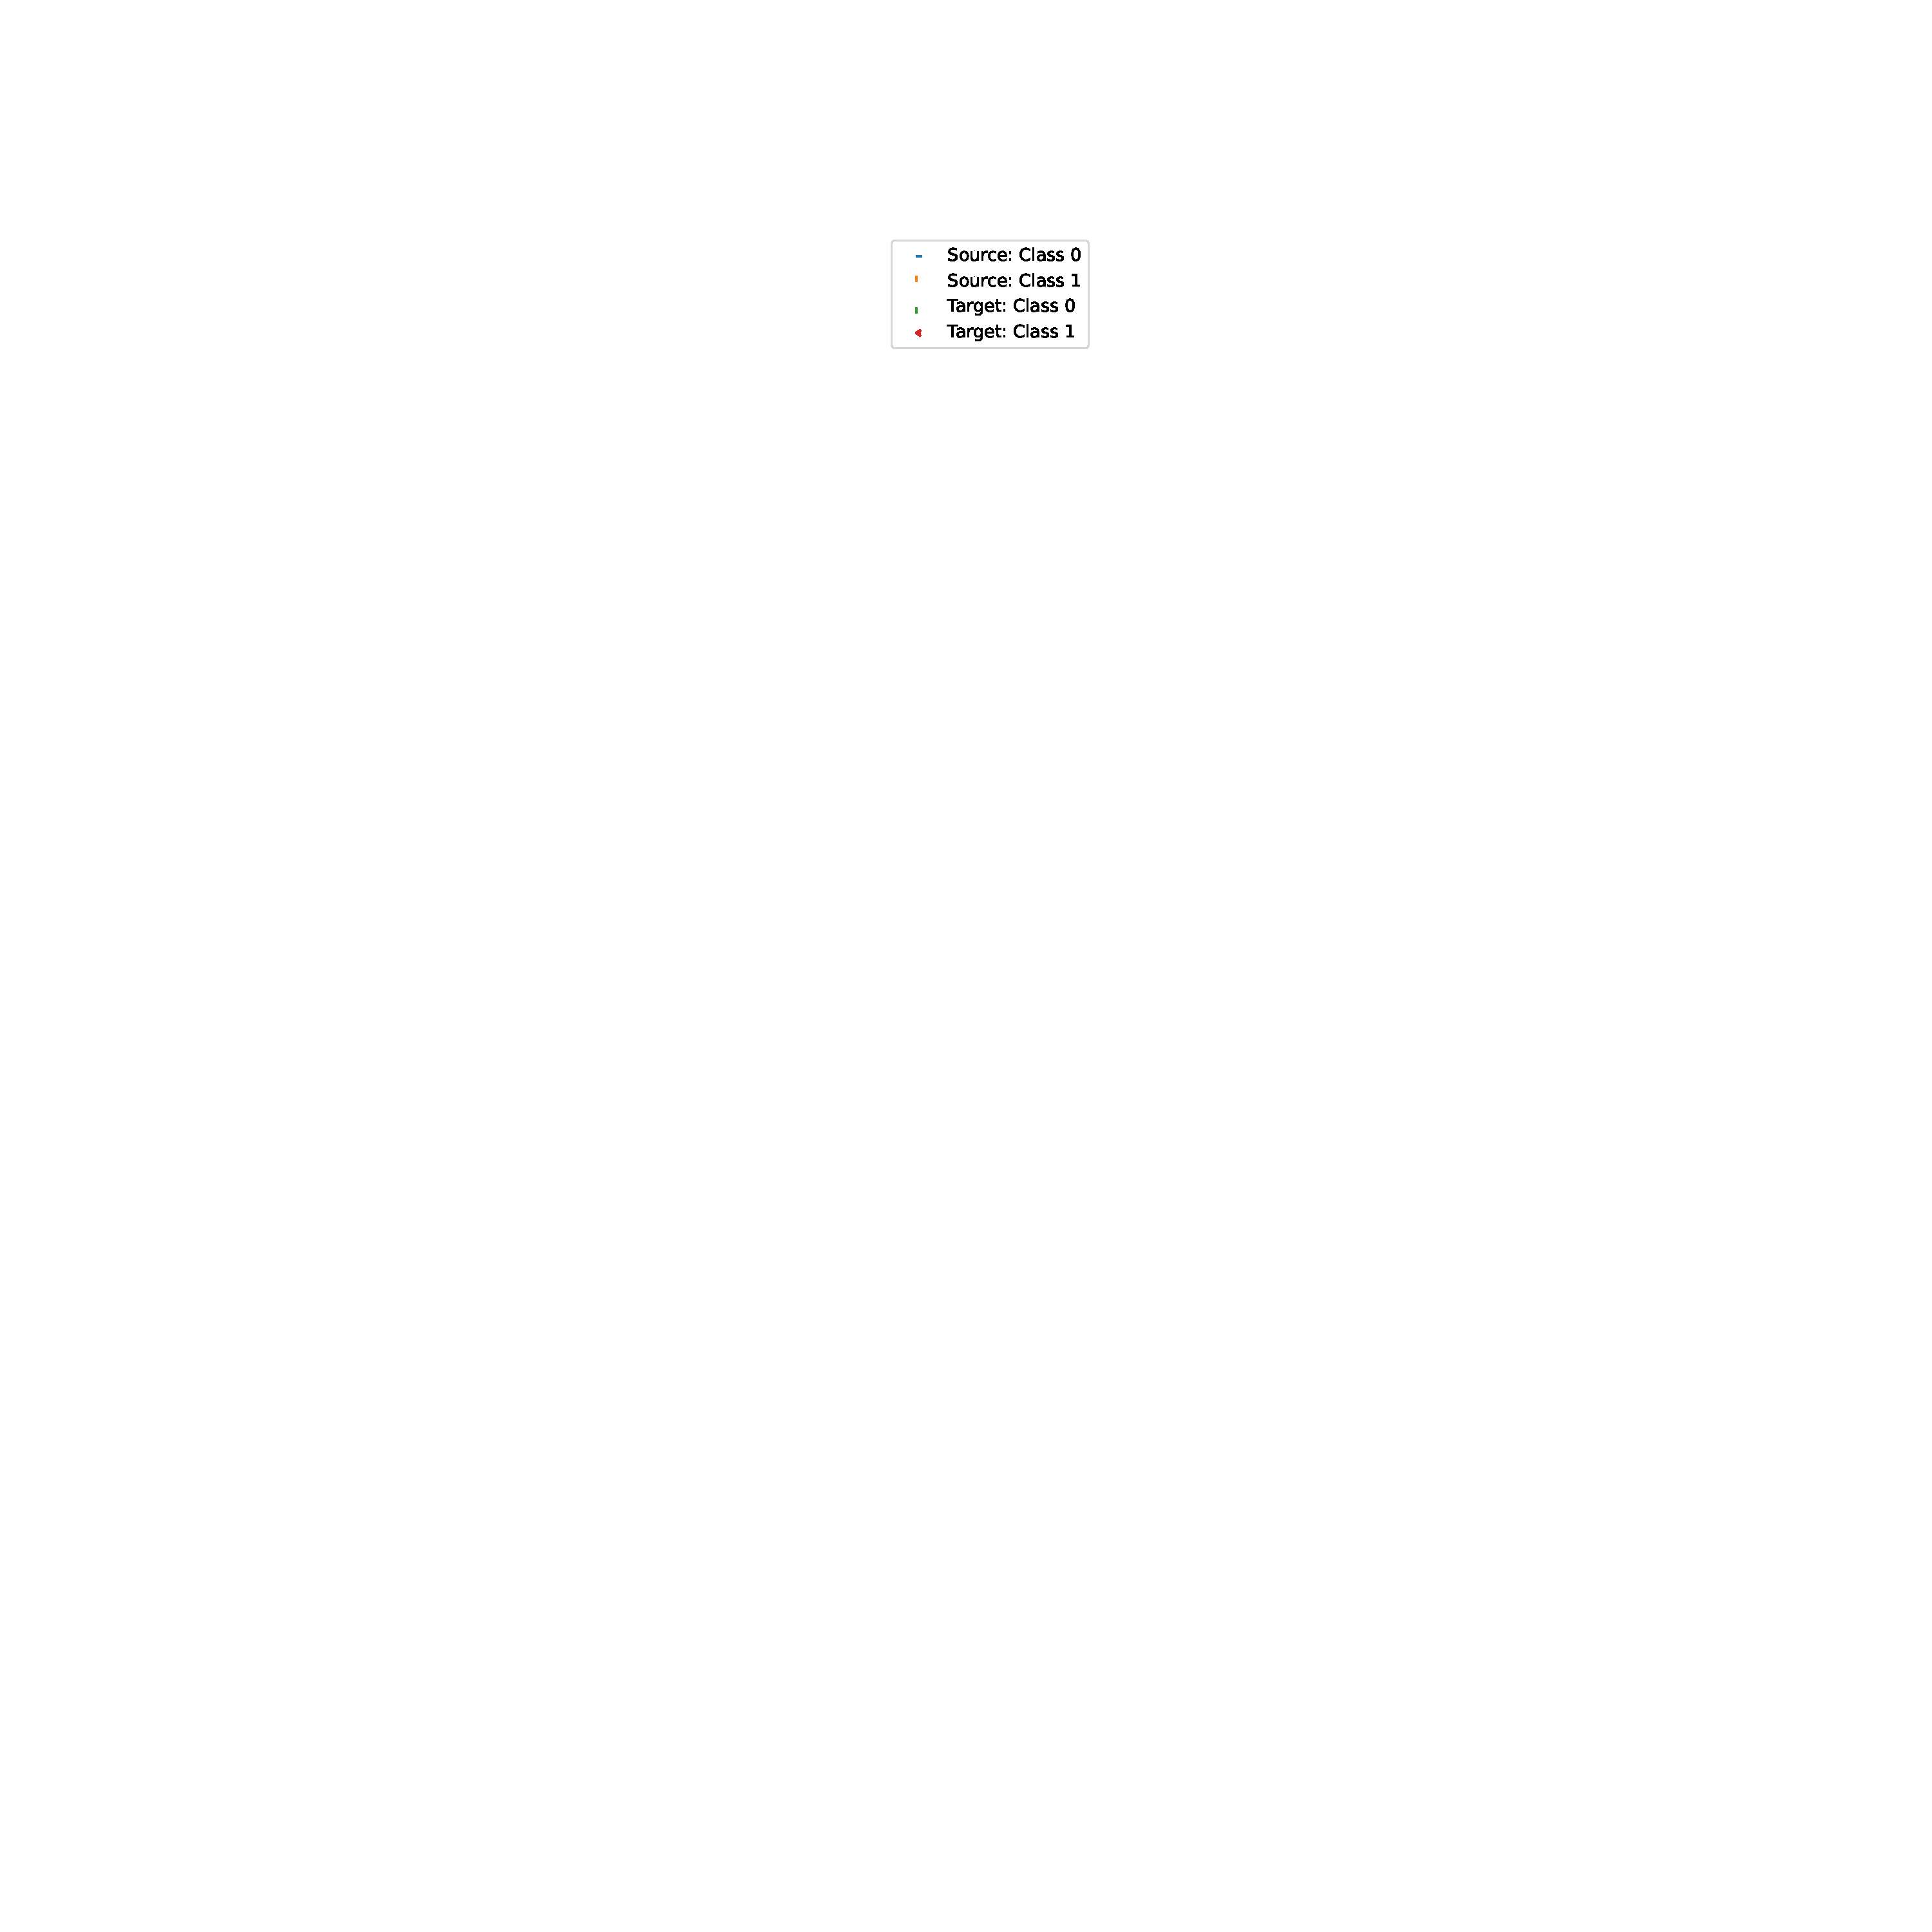
\includegraphics[width=.15\textwidth]{labeled_vs_unlabeled_point_cloud/legend.pdf}


  \caption{Data distribution: Influence of GAMMA on model training, with GAMMA = 0.1 (top), GAMMA = 0,5 (middle), GAMMA = 30 (bottom)}
  \label{fig:point_cloud_mmd}
\end{figure}
\FloatBarrier 





\begin{figure}[p]
  \centering
  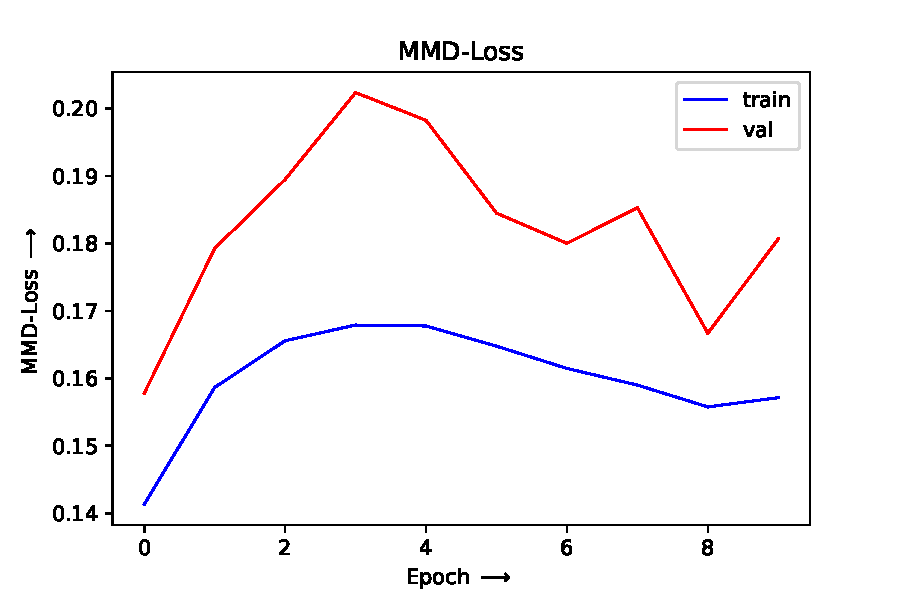
\includegraphics[width=.45\textwidth]{GAMMA_plot/mmd_loss_0_1.pdf}
  \hspace{.3cm}
  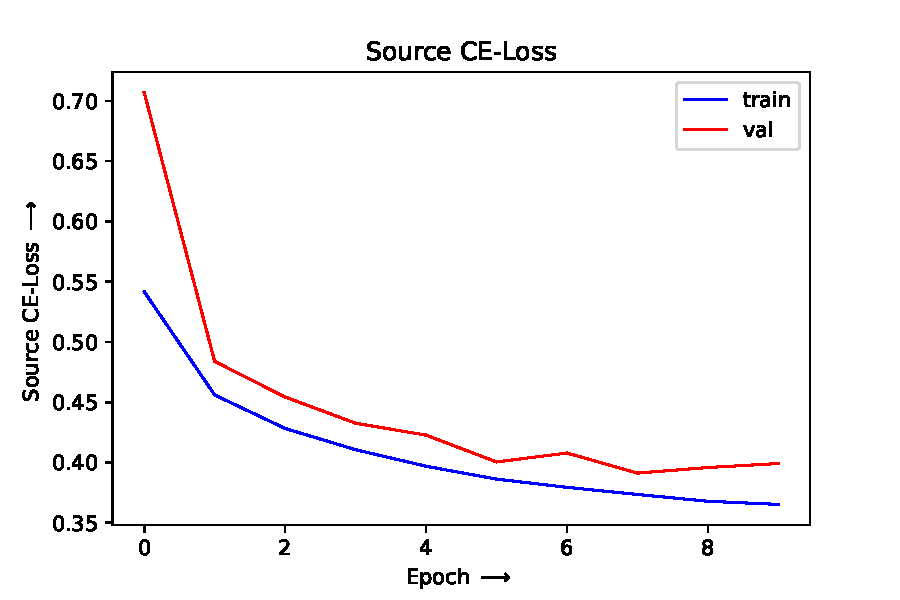
\includegraphics[width=.45\textwidth]{GAMMA_plot/source_ce_loss_0_1.pdf}

  \vspace{.3cm}

  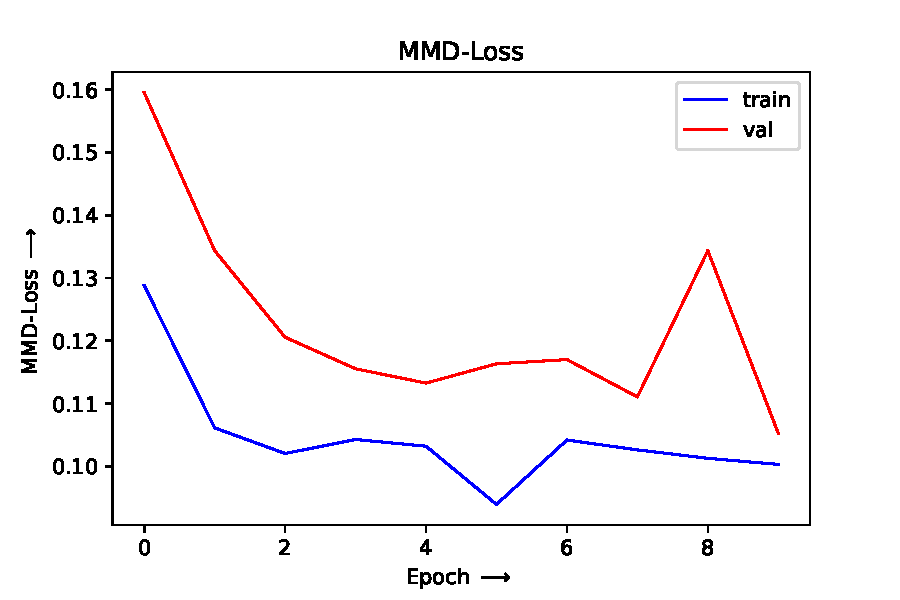
\includegraphics[width=.45\textwidth]{GAMMA_plot/mmd_loss_0_5.pdf}
  \hspace{.3cm}
  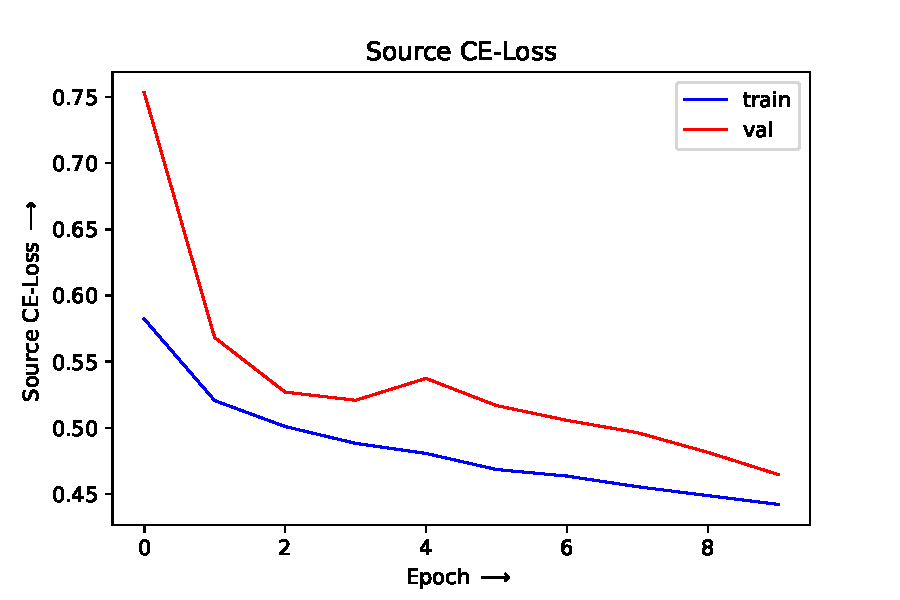
\includegraphics[width=.45\textwidth]{GAMMA_plot/source_ce_loss_0_5.pdf}

  \vspace{.3cm}

  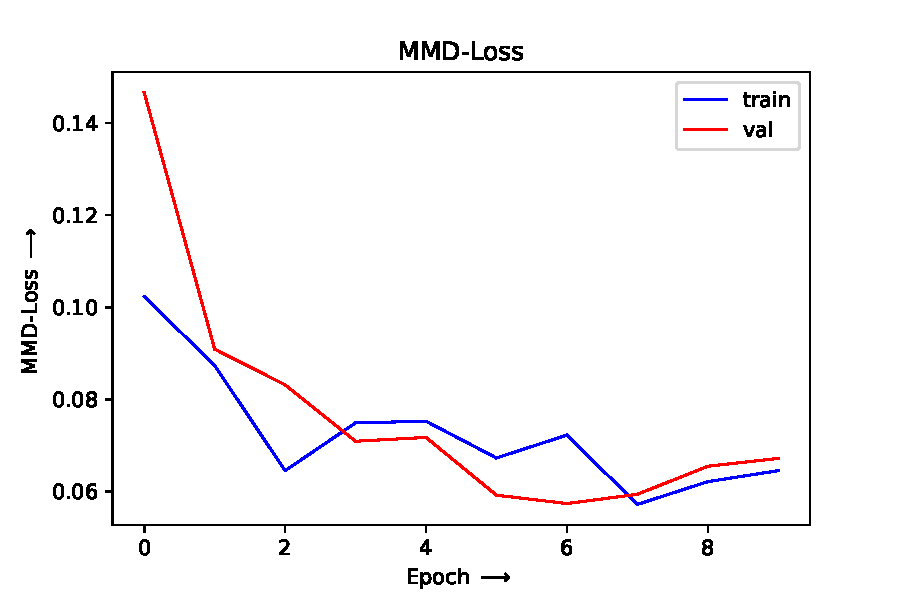
\includegraphics[width=.45\textwidth]{GAMMA_plot/mmd_loss_30.pdf}
  \hspace{.3cm}
  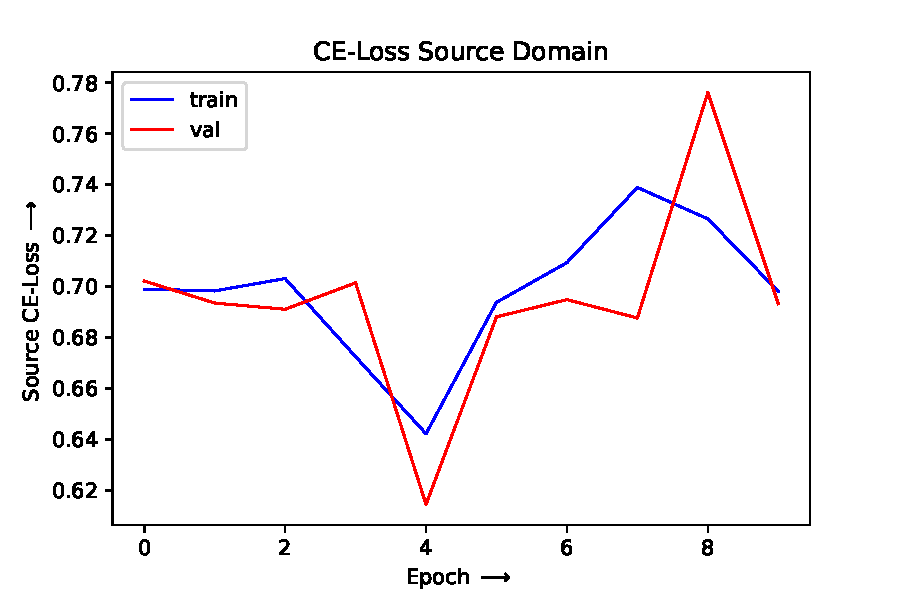
\includegraphics[width=.45\textwidth]{GAMMA_plot/source_ce_loss_30.pdf}

  \caption{MMD and Source CE-Loss curves: Influence of GAMMA on model training, with GAMMA = 0.1 (top), GAMMA = 0,5 (middle), GAMMA = 30 (bottom)}
  \label{fig:learning_curves_influence_mmd_feature_extractor}
\end{figure}
\FloatBarrier 







Just when the GAMMA is chosen correctly the source cross-entropy and MMD loss can be reduced. Is the GAMMA too big or too small the optimization just focuses on one of the two losses. In the case of a big GAMMA, the model does not learn to separate between classes, but to reduce the distance between the samples of all classes and domains. If GAMMA is picked to small the model is able to predict the the labels for the source domain samples accurately but can not transfer that knowledge on the target domain. 






\subsection{Labeled vs. unlabeled MMD loss} \label{sec:Differences of labeled and unlabeled MMD loss}

The idea behind domain adaption is to aggregate knowledge while solving one problem and transferring that knowledge to another problem. For this reason in domain adaption tasks the goal is to restrict the supervised learning solely on the source domain data. Section \ref{sec:Balancing Cross-Entropy and MMD loss} describes that applying the MMD loss in general helps to reduce the domain discrepancy. Since the target labels are unknown the intra and inter class distance between source and target samples is minimized. Obviously this also reduces the separability of classes in the source and target domain. In the literature domain adaption approaches which use a small amount of the target domain labels are known under the name "Few-shot transfer learning" \cite{WU2020}. Similarly in this section the effect of including a few target labels into the training is analysed. The cross-entropy loss is still restricted to source samples and corresponding labels only. Solely the MMD loss is allowed to use the target labels. This allows to separately calculate the distance between source and target samples of similar and of different classes. The labeled MMD loss optimizes the model such, that the intra class distance between the domains is maximized and the inter class distance is minimized. The domain discrepancy is reduced by minimizing the the inter class distance. The separability is improved by maximizing the the intra class distance. In parallel the training still includes the source cross-entropy loss in order to improve the source domain classification task. The hyperparameter GAMMAIntraClass and GAMMAInterClass are used to balance the training scope of reducing the inter class distance, maximizing the intra class distance and improving the source domain classification problem:

\begin{equation}
\begin{split}
    TotalMMDLoss = GAMMAIntraClass * MMDLossIntraClass\\ + GAMMAInterClass * MMDLossInterClass + CELoss
\end{split}
\end{equation}

 The MMD loss which includes the target labels is called "labeled MMD loss" and otherwise "unlabeled MMD loss". For the evaluation the model optimization method described in section \ref{sec:Balancing Cross-Entropy and MMD loss} reused. Fig. \ref{fig:point_cloud_labeled_unlabeled_mmd} visualizes the distribution of the latent feature representation distribution of the source and target samples within the penultimate hidden layer. Throughout the training both MMD losses reduce the domain discrepancy and increase the separability between classes of both domains. When applying the labeled MMD loss the distance between classes of both domains is bigger compared to the unlabeled MMD loss. This makes classification problem easier and besides that the trivial solution in which the latent feature representation of all samples collapse at one point is prevented. On the other hand one has to remember that target labels of just 20 percent are known. Therefore, the labeled MMD loss can just be applied on a small subset of coupled source and target samples. In comparison the unlabeled MMD loss can be applied on the whole dataset.




\begin{figure}[p]
  \centering
  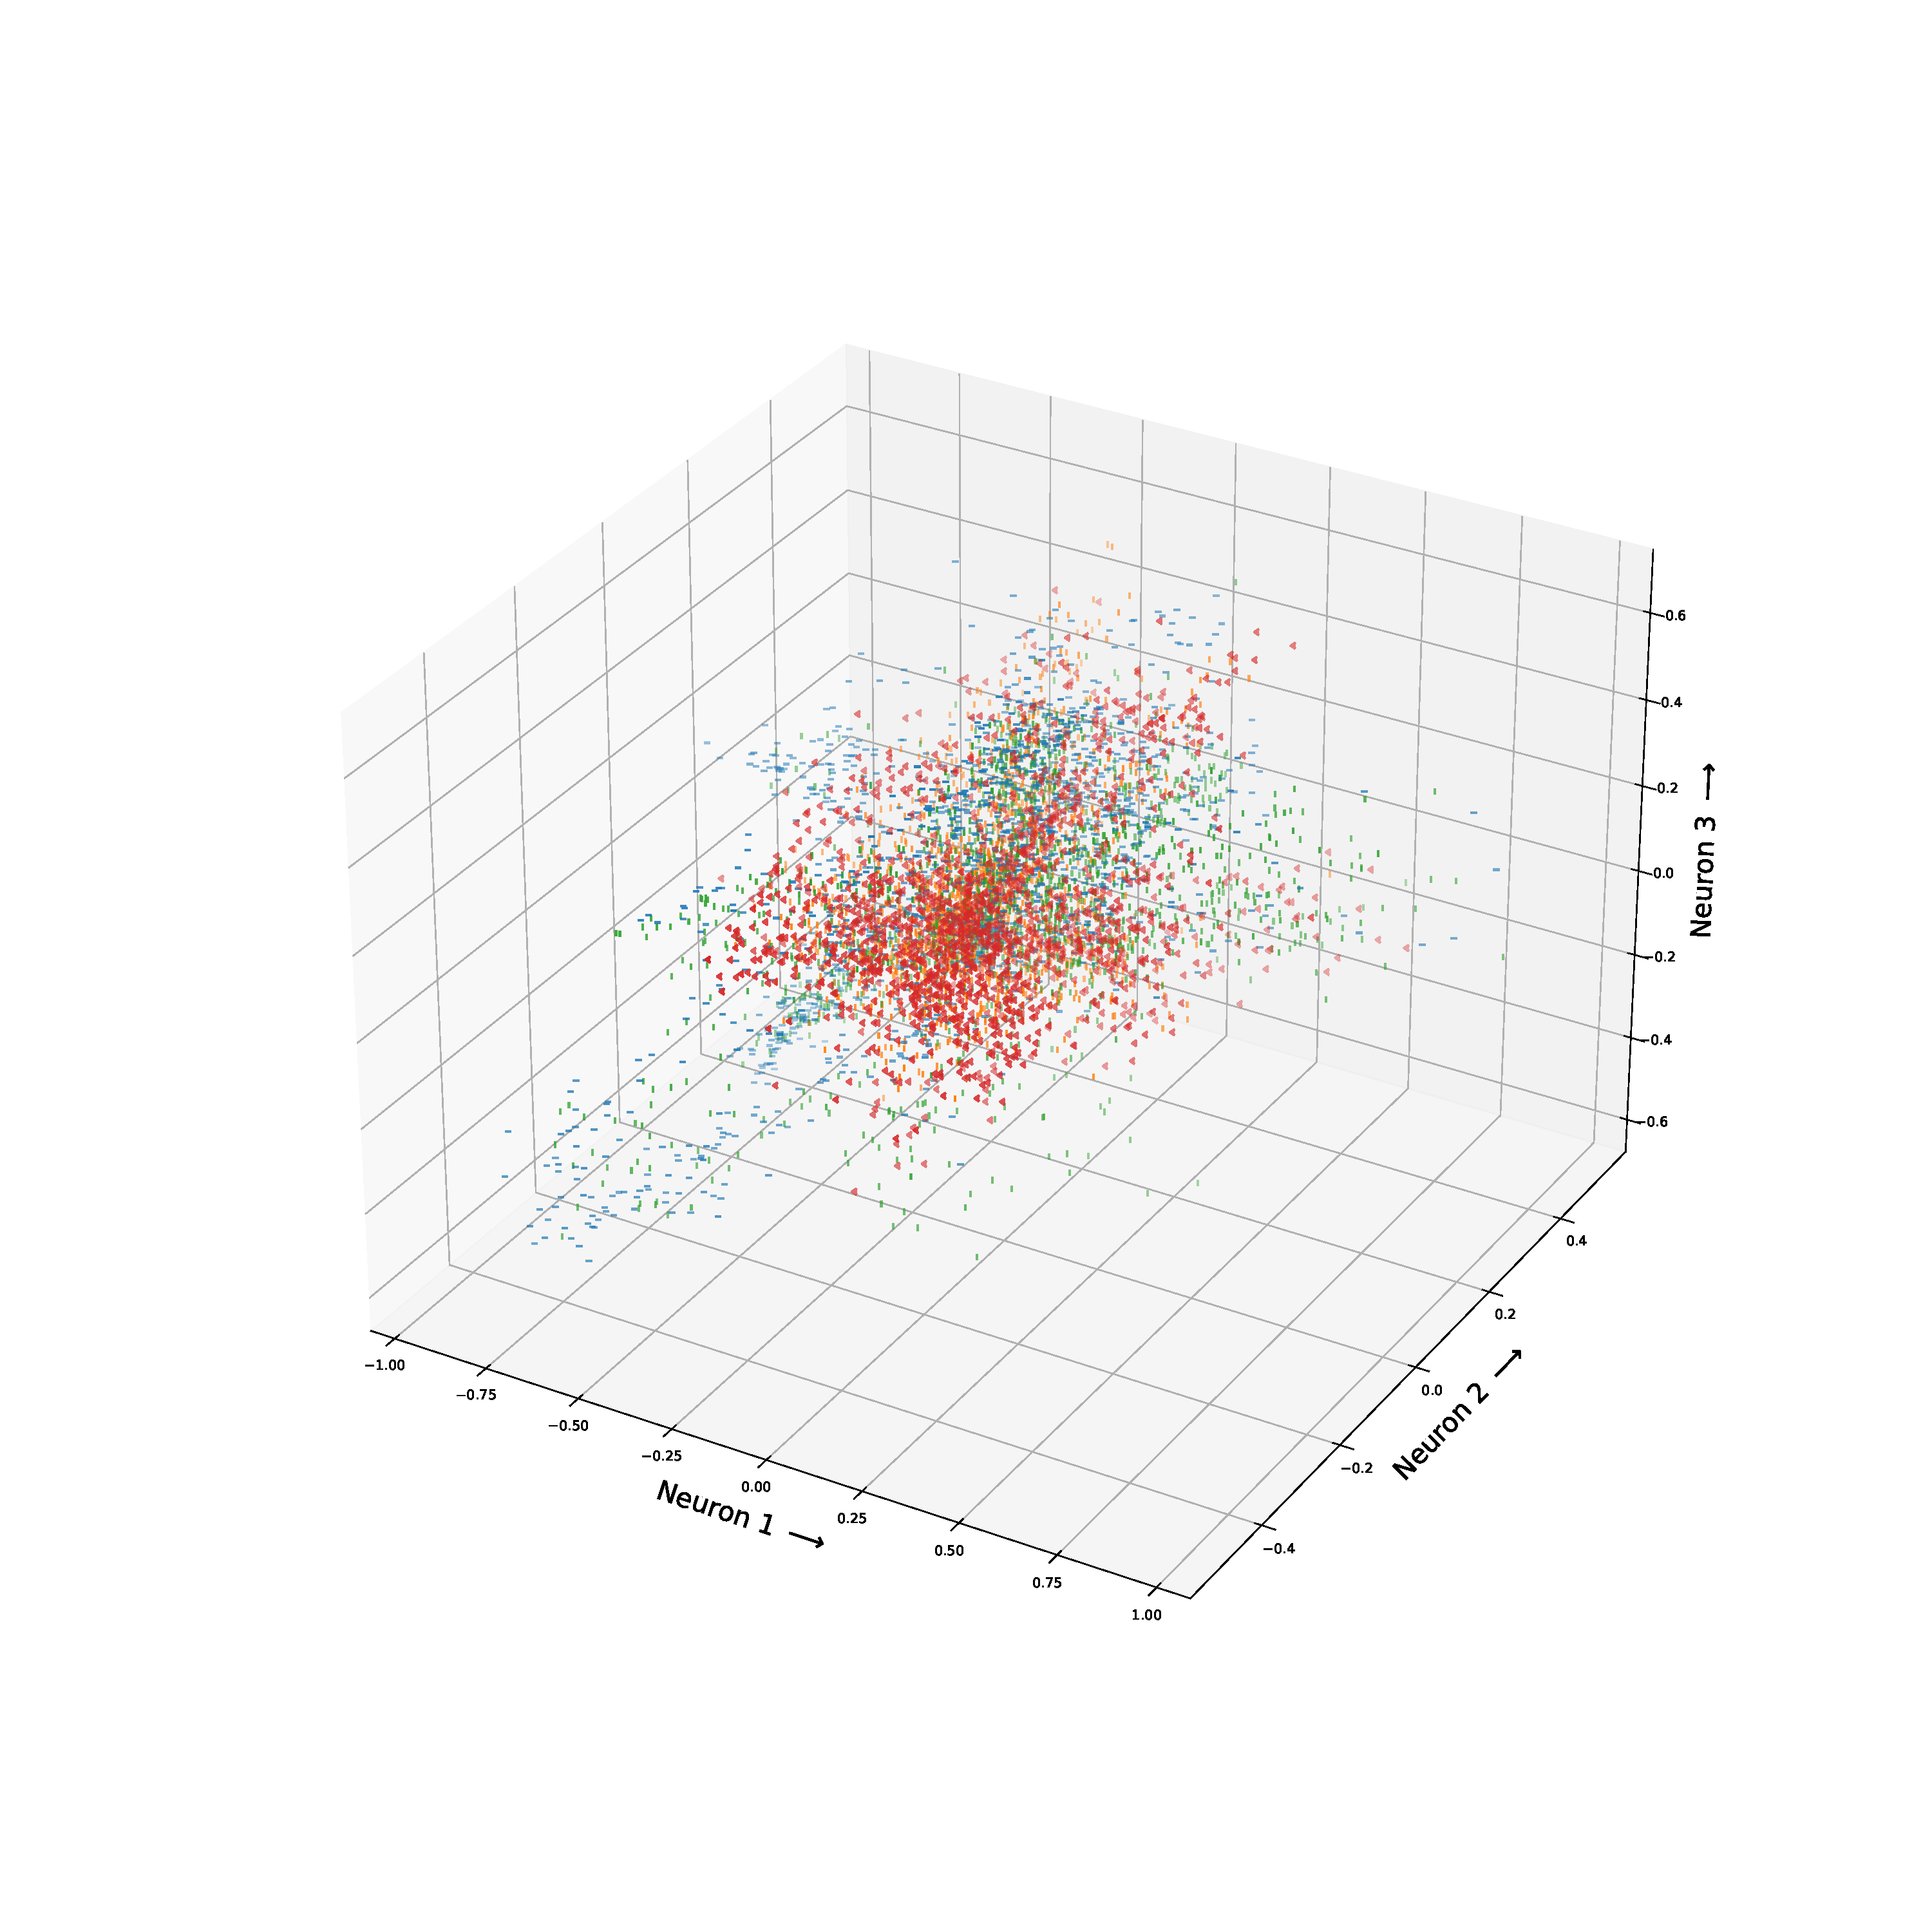
\includegraphics[width=.44\textwidth]{labeled_vs_unlabeled_point_cloud/labeled_mmd_epoch0.pdf}
  \hspace{.3cm}
  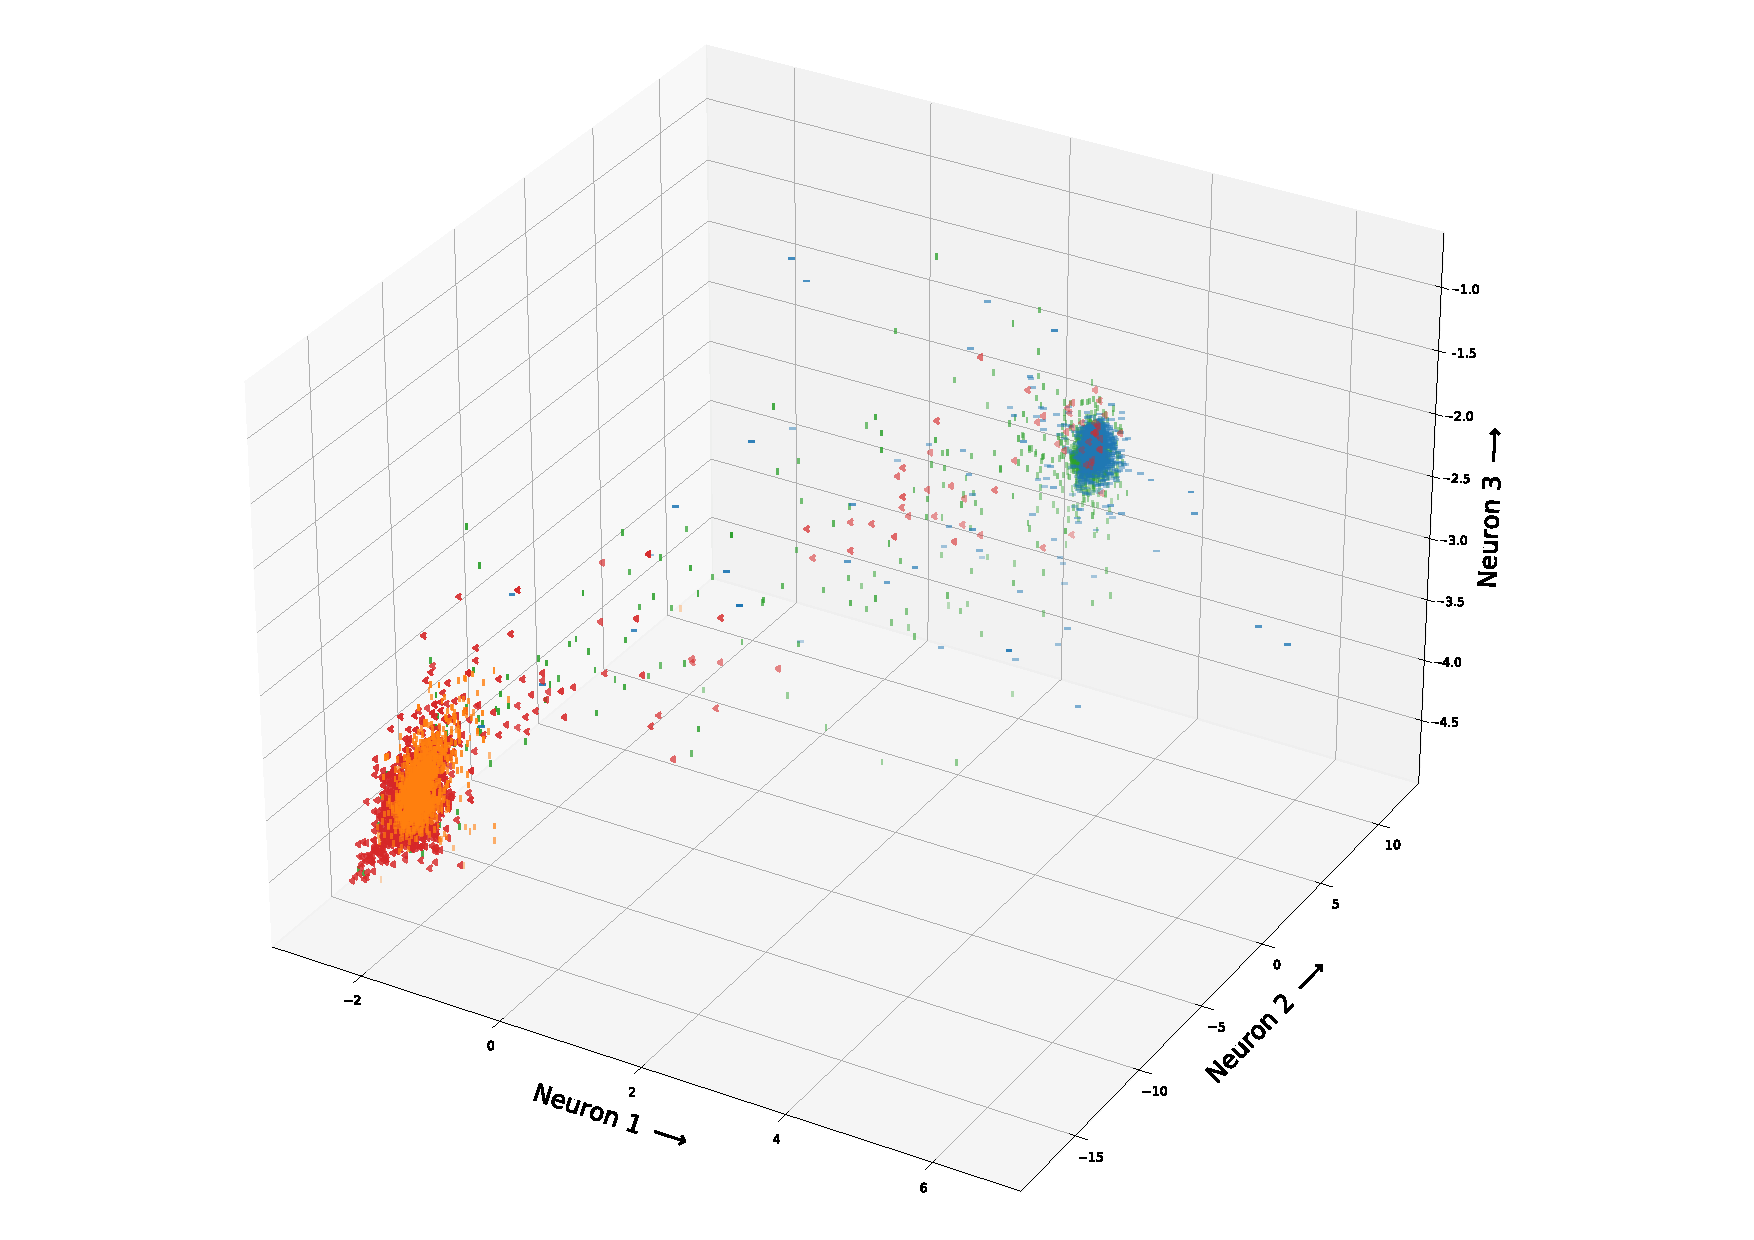
\includegraphics[width=.44\textwidth]{labeled_vs_unlabeled_point_cloud/labeled_mmd_epoch6.pdf}

  \vspace{.1cm}

  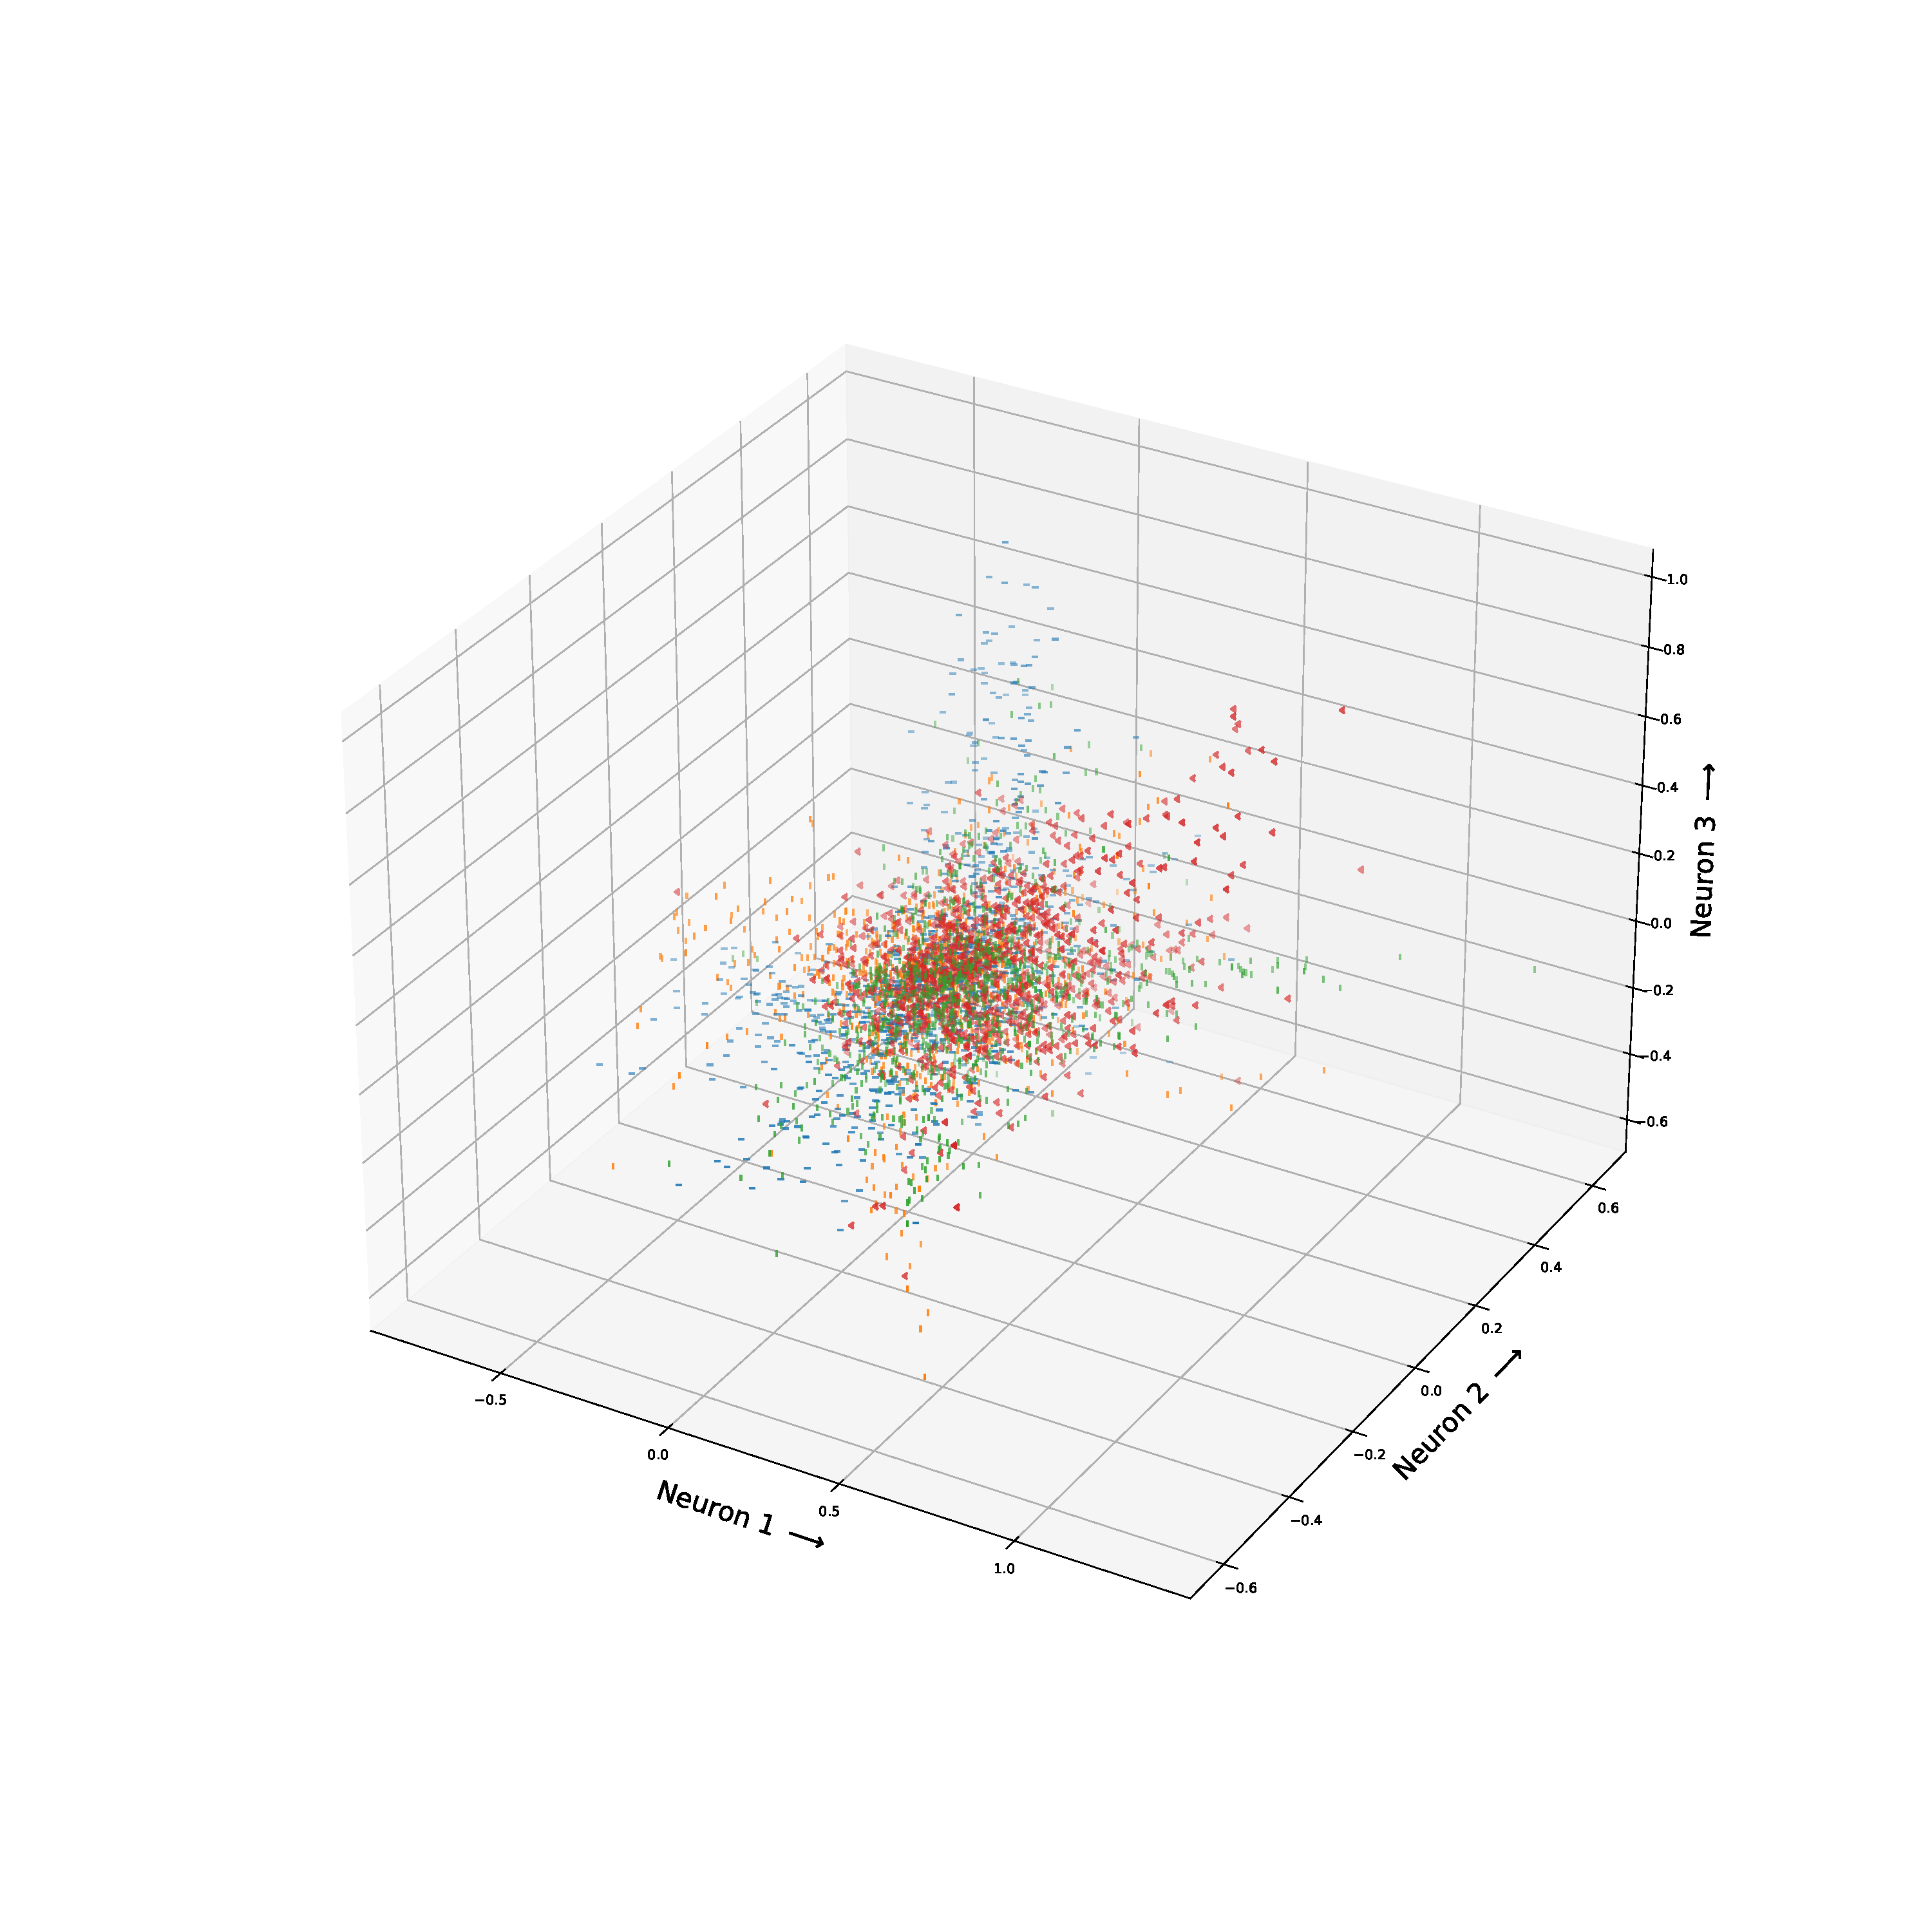
\includegraphics[width=.44\textwidth]{labeled_vs_unlabeled_point_cloud/mmd_epoch0.pdf}
  \hspace{.1cm}
  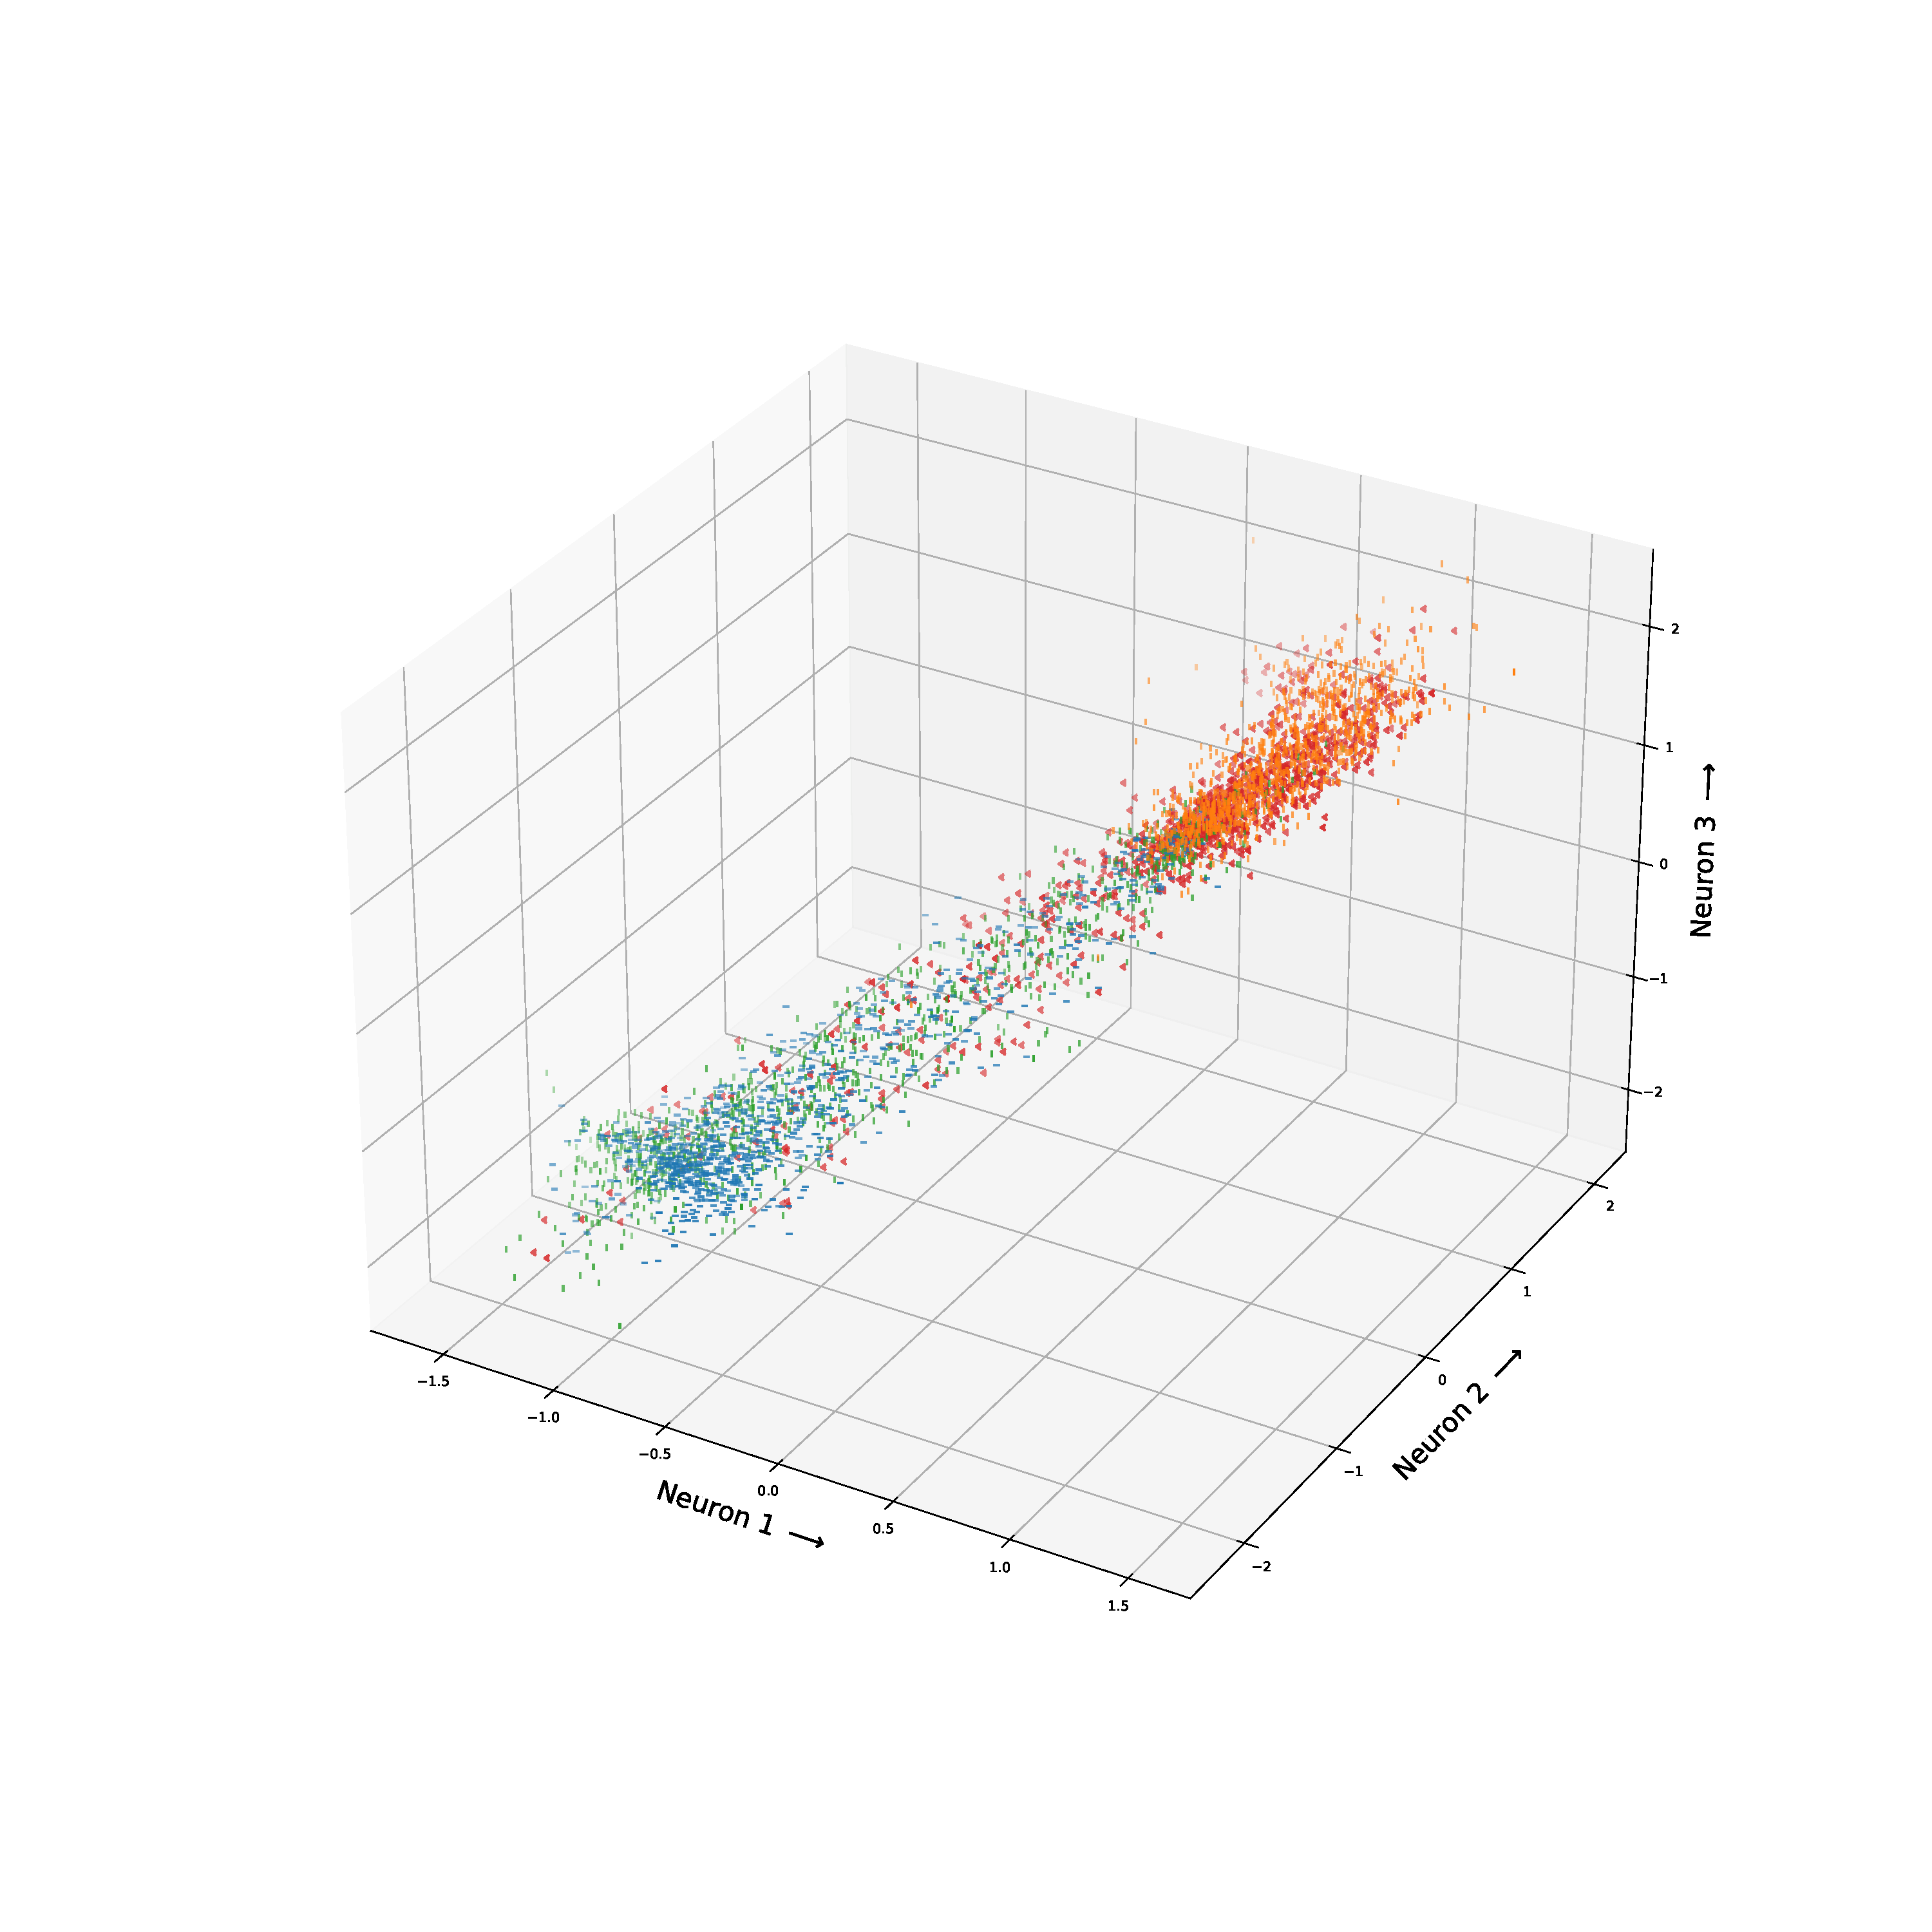
\includegraphics[width=.44\textwidth]{labeled_vs_unlabeled_point_cloud/mmd_epoch6.pdf}

  \vspace{.1cm}
  
  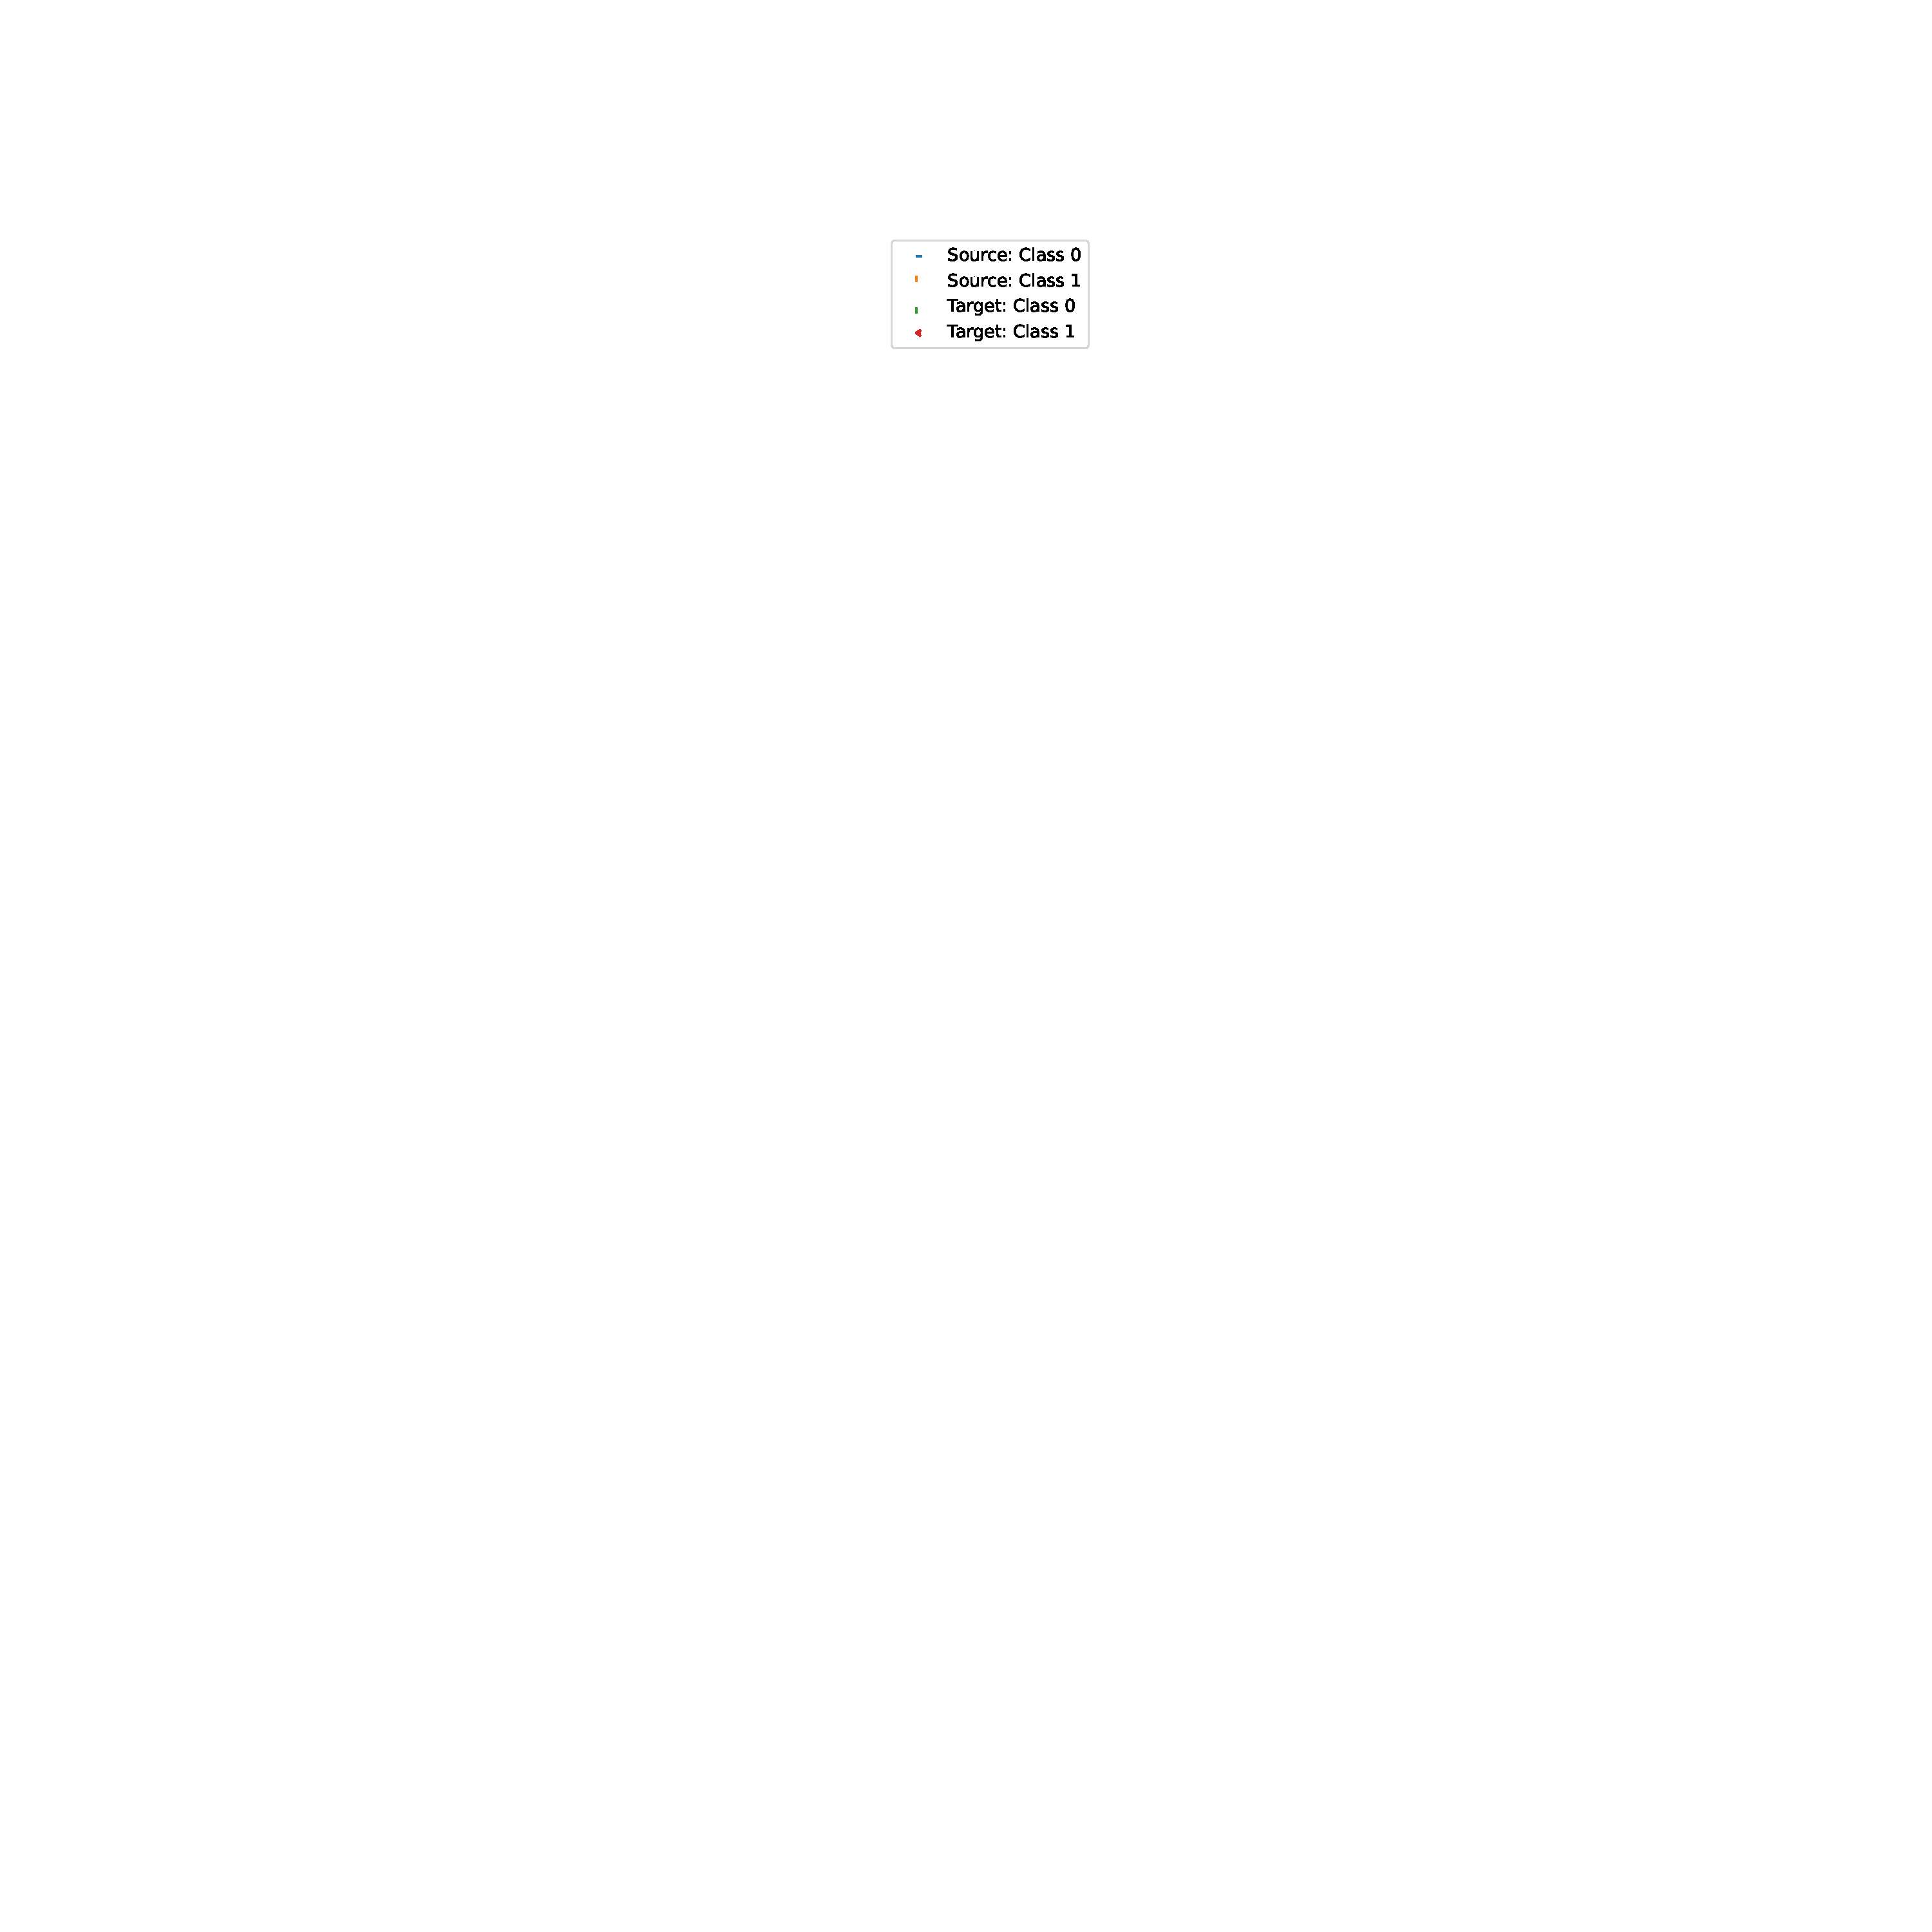
\includegraphics[width=.15\textwidth]{labeled_vs_unlabeled_point_cloud/legend.pdf}


  \caption{Data distribution: labeled (top) vs. unlabeled MMD (bottom) at epoch 0 (left) and epoch 6 (right)}
  \label{fig:learning_curves_influence_mmd_feature_extractor}
\end{figure}
\FloatBarrier 


\subsection{Influence of latent feature space choice in MMD loss}
This section analyses the efficiency of reducing the domain discrepancy with varying MMD losses including features from different hidden layers. Fig. \ref{fig:visualization_extraction_loss} visualizes the calculation of two MMD losses by extracting different latent features from the classifier and the CNN. The evaluation is based on the model presented in fig. \ref{fig:model_latent_feature_space_test_dumm}. The model is trained in three different phases. During the MMD-Loss phase a weighted average of the MMD and cross entropy loss and during the CE-Loss phase just a cross entropy loss is applied. In both phases ADAM is used as optimizer with gamma1 = 0.9, gamma2 = 0.99 and a learning rate of 1e-2 for the CNN and 1e-4 for the classifier. The "regular FC MMD" loss calculates the source and target discrepancy from the latent features in the fully connected layers of the classifier. The "regular FC + CNN MMD" loss additionally considers the feature maps extracted right after the convolutional layers in the CNN. 

\begin{figure}[htpb]
  \centering
  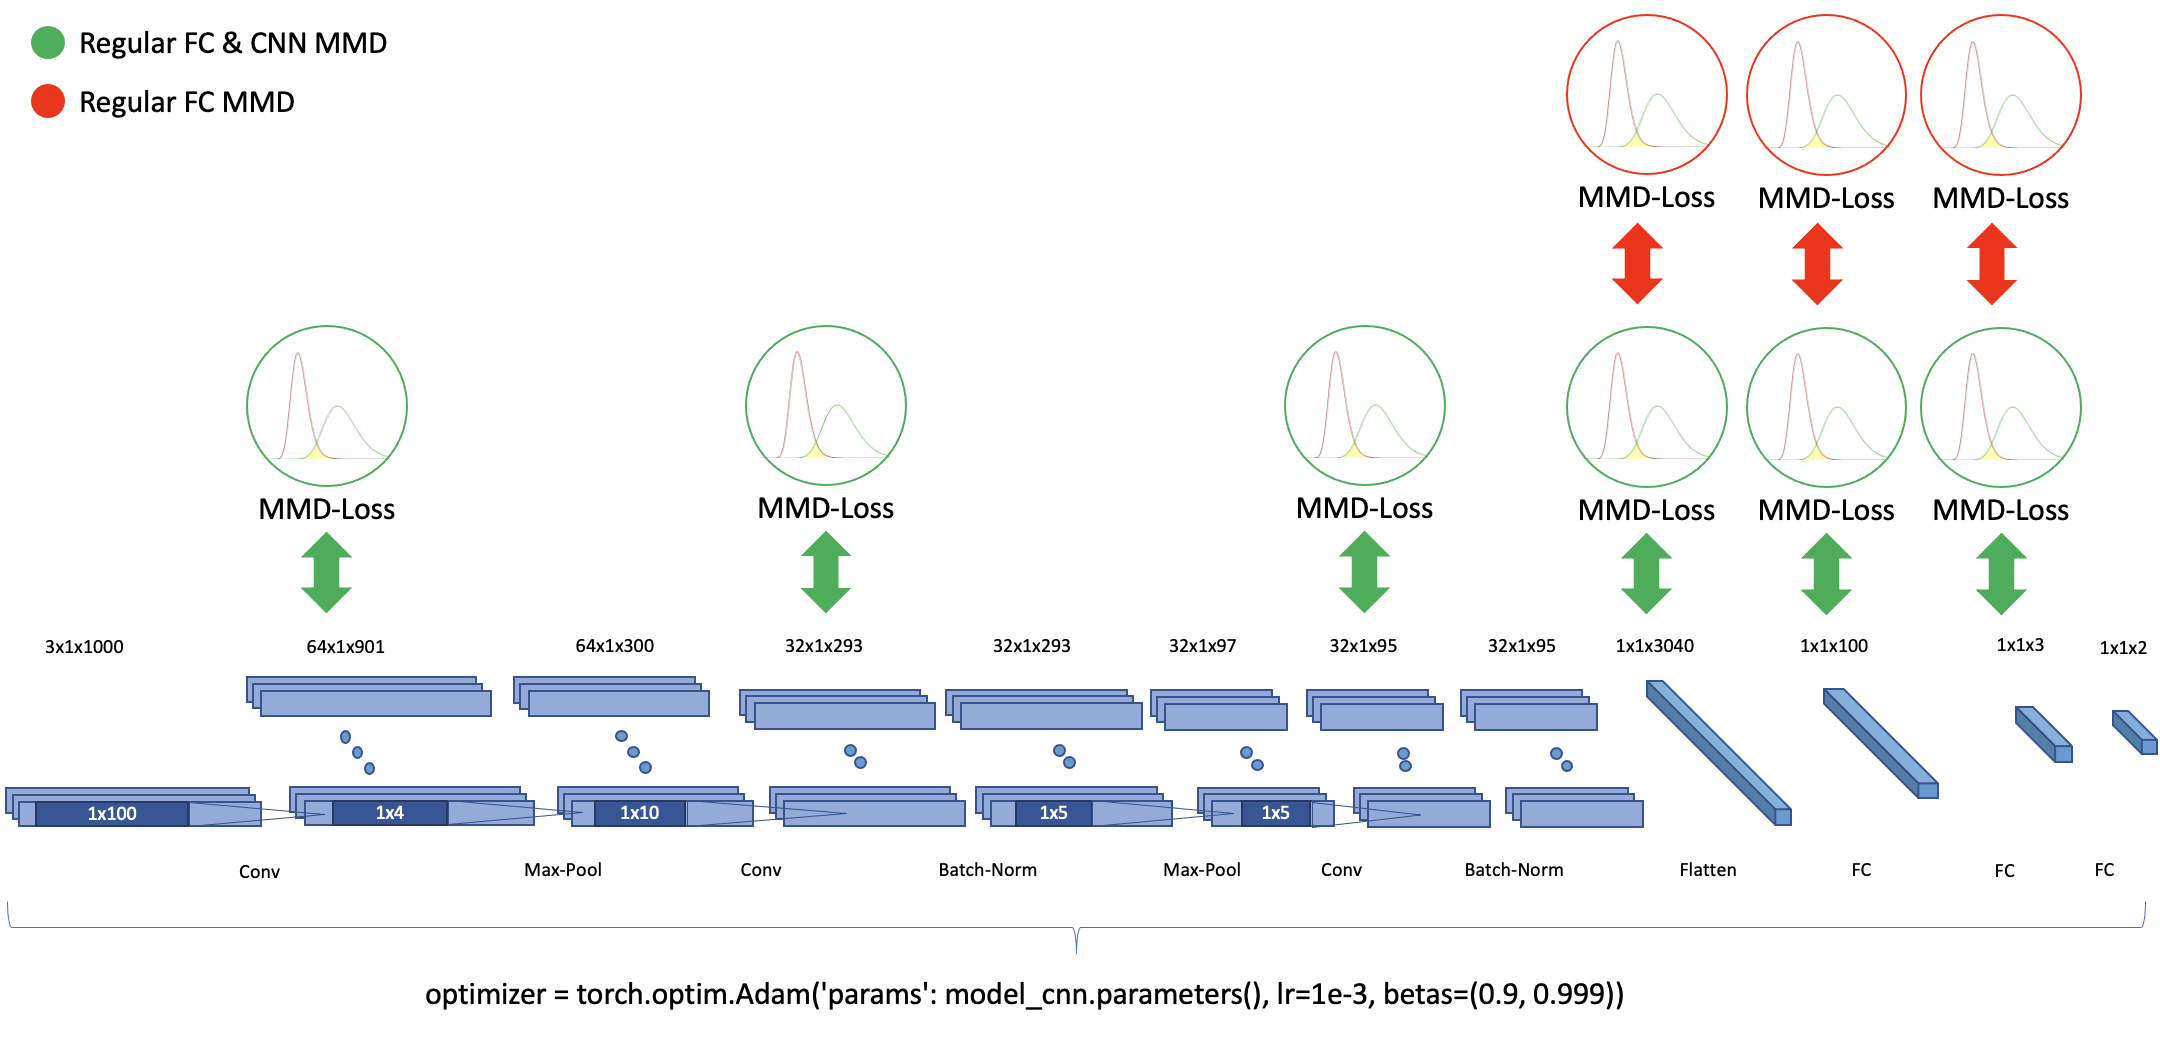
\includegraphics[width=1\textwidth]{visualization_extraction_loss.png}
  \caption {Visualization: extraction MMD loss in different hidden layers of neural network as well as CE loss} \label{fig:visualization_extraction_loss}
\end{figure}



\begin{figure}[htpb]
  \centering
  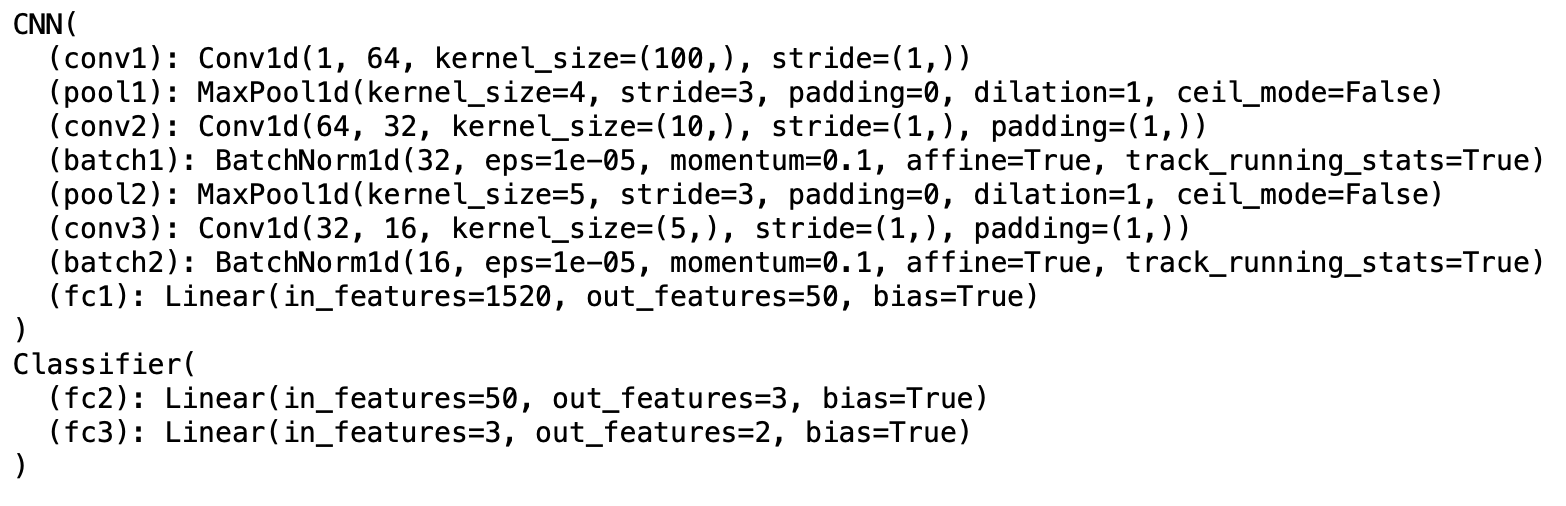
\includegraphics[width=1.1\textwidth]{model_latent_feature_space_test_dumm}
  \caption {Model architecture used for evaluating the effect of including different classifier and CNN latent feature spaces in the MMD loss} \label{fig:model_latent_feature_space_test_dumm}
\end{figure}

The development of the accuracy, the source cross-entropy and MMD loss during the training process are shown in fig. \ref{fig:accuracy_cnn_and_no_cnn_mmd} and fig. \ref{fig:loss_cnn_and_no_cnn_mmd}. The accuracies in source and target domain tend to be a little higher when including the CNN feature maps into the MMD loss. The main advantage of including the CNN feature maps is the increased stability of the training. The MMD and cross entropy loss as well as the accuracies converge faster and smoother.






\begin{figure}[p]
  \centering
  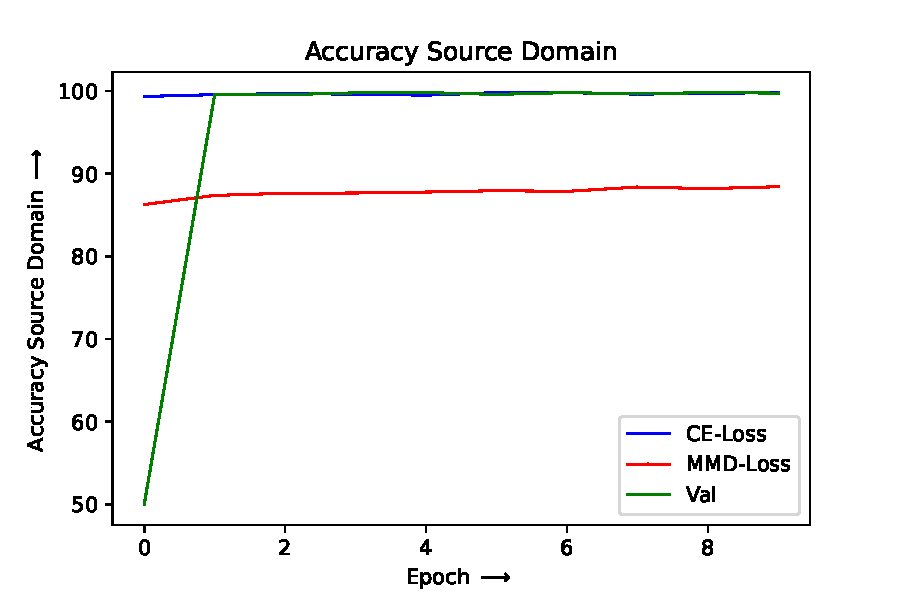
\includegraphics[width=.47\textwidth]{plots_CNN_MMD/Accuracy_Source_Domain_CNN_MMD.pdf}
  \hspace{.3cm}
  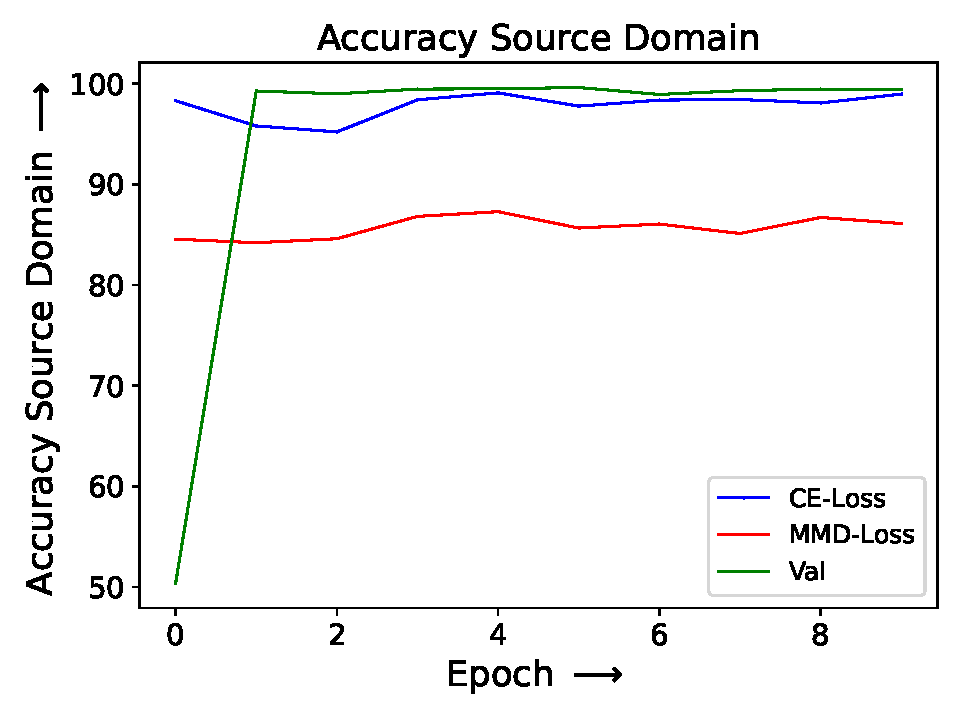
\includegraphics[width=.47\textwidth]{plots_CNN_MMD/Accuracy_Source_Domain_FC_MMD.pdf}

  \vspace{.1cm}

  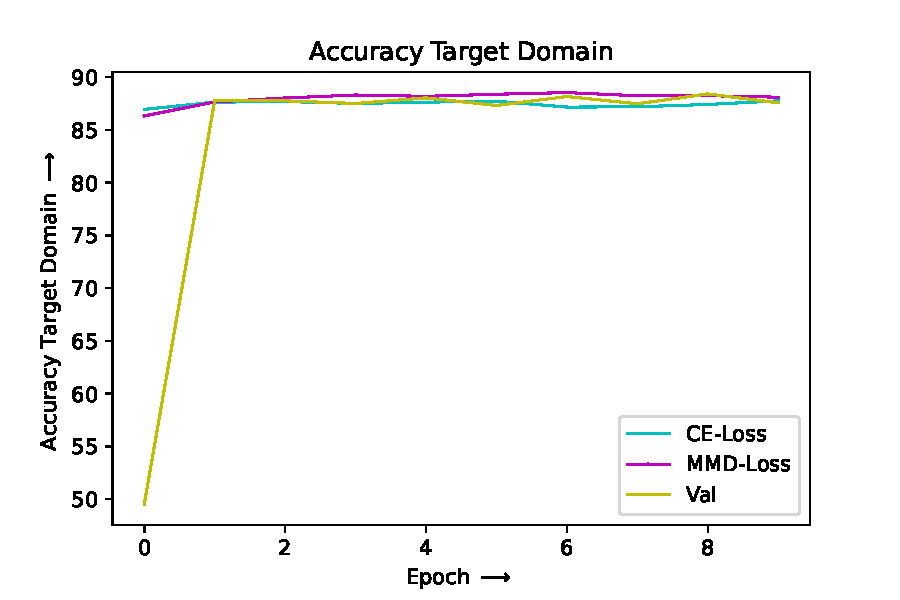
\includegraphics[width=.47\textwidth]{plots_CNN_MMD/Accuracy_Target_Domain_CNN_MMD.pdf}
  \hspace{.1cm}
  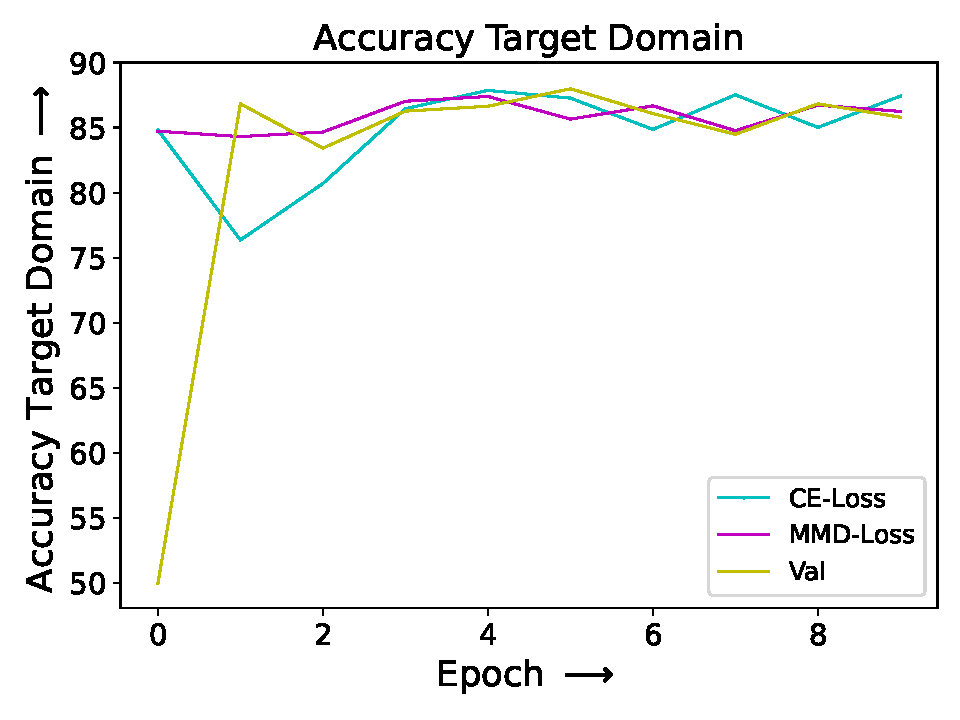
\includegraphics[width=.47\textwidth]{plots_CNN_MMD/Accuracy_Target_Domain_FC_MMD.pdf}

  \caption{Accuracy curves of regular CNN MMD Loss (left) and regular FC MMD Loss (right)}
  \label{fig:accuracy_cnn_and_no_cnn_mmd}
\end{figure}
\FloatBarrier 




\begin{figure}[p]
  \centering
  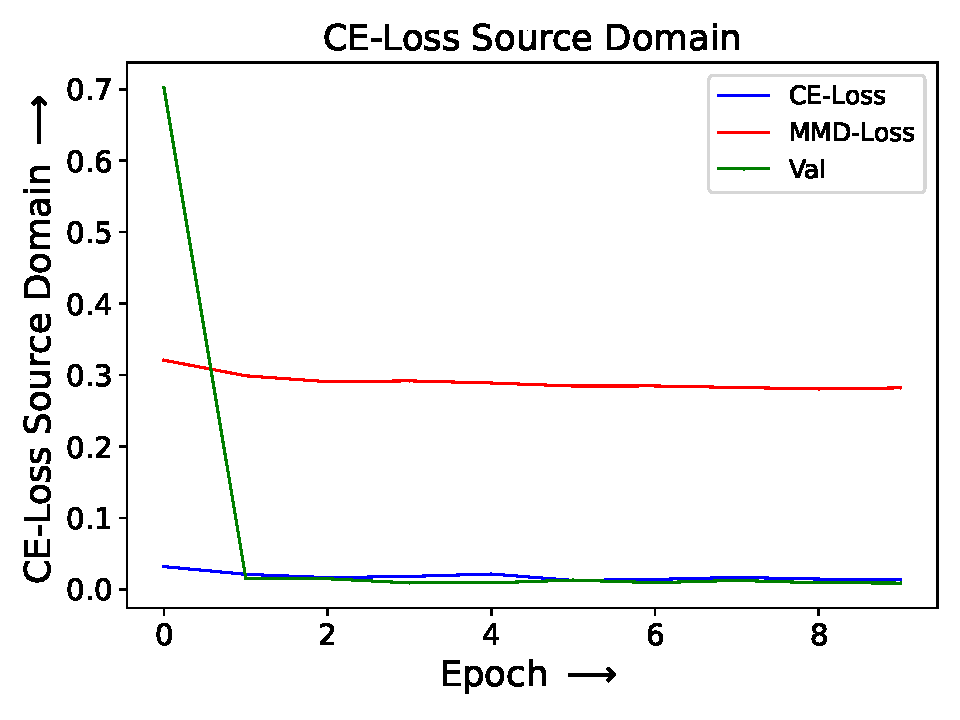
\includegraphics[width=.47\textwidth]{plots_CNN_MMD/CE_Loss_Source_Domain_CNN_MMD.pdf}
  \hspace{.3cm}
  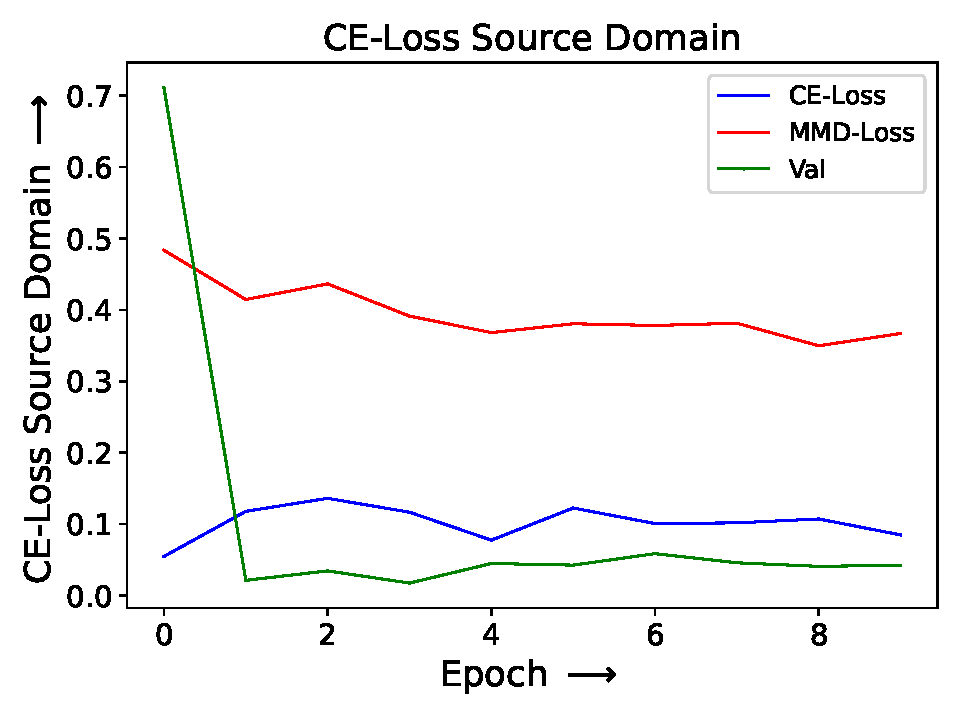
\includegraphics[width=.47\textwidth]{plots_CNN_MMD/CE_Loss_Source_Domain_FC_MMD.pdf}

  \vspace{.1cm}

  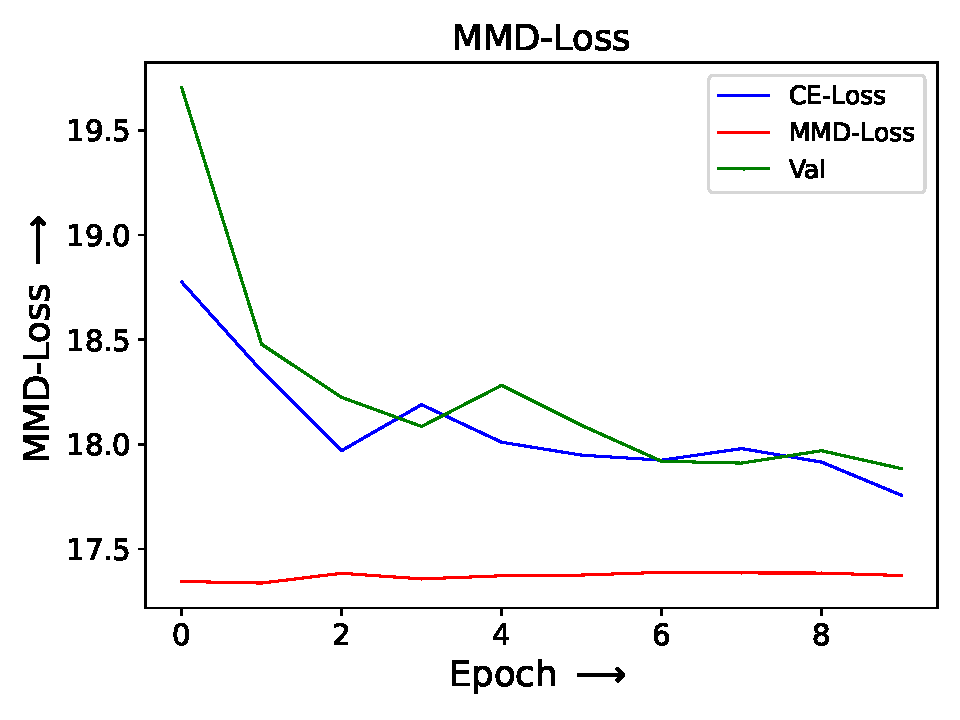
\includegraphics[width=.47\textwidth]{plots_CNN_MMD/MMD_Loss_CNN_MMD.pdf}
  \hspace{.1cm}
  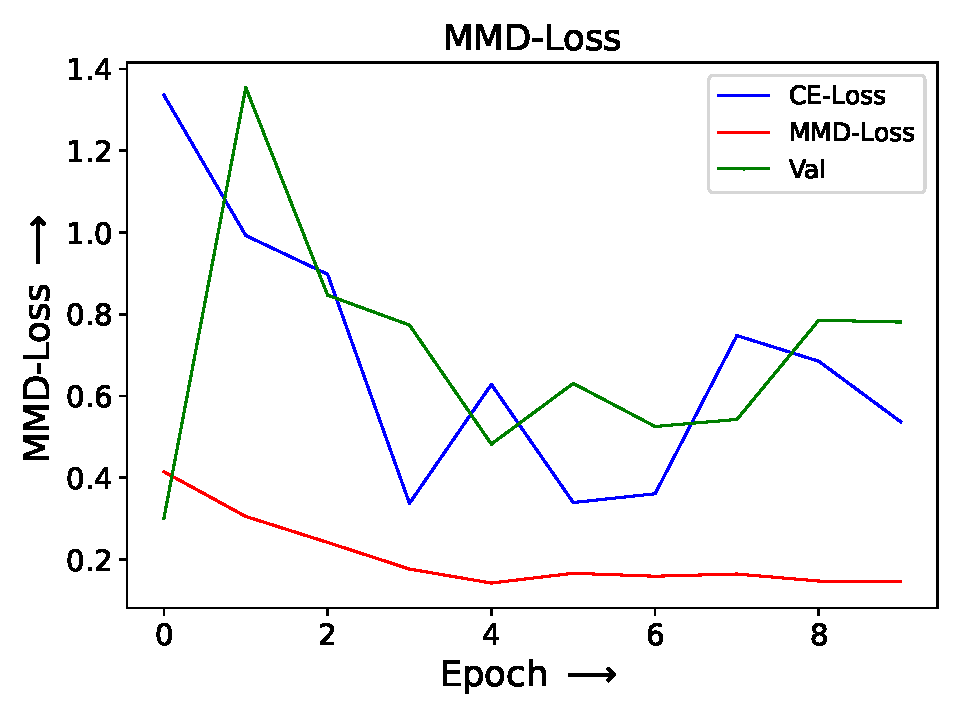
\includegraphics[width=.47\textwidth]{plots_CNN_MMD/MMD_Loss_FC_MMD.pdf}

  \caption{Loss curves of regular CNN MMD loss (left) and regular FC MMD loss(right)}
  \label{fig:loss_cnn_and_no_cnn_mmd}
\end{figure}
\FloatBarrier 



By passing data through the model, features with varying levels of abstraction are extracted. From the just presented results it seems reasonable to supervise the domain discrepancy in feature spaces of different abstraction levels. Generally deeper layers in neural network extract rather more task specific features. Therefore deeper layers often suffer more from domain-dependencies. Since each hidden layer's output influences subsequent layers, it makes sense to apply the MMD loss early in the network. Reducing the domain discrepancy in shallow layer makes the network extract more domain-invariant features in deeper layers. Without intervening in early layers the domain discrepancy gets more difficult to solve in deeper layers. Reducing the domain discrepancy in the final layers of the model leads to an less stable optimization problem. In this case the MMD and source cross-entropy loss show tendencies to work against each other. In these cases the optimization seems to focus just on one optimization goal and forgetting the others. Throughout the different training phases these goals change. The total optimization therefore fluctuates a little more throughout the training phases of one epoch and also the epochs themselves. The models performance sometimes breaks down after quiet some epochs of constant performance increases. One has to remember calculating the regular FC + CNN MMD loss is quiet expansive since the features extracted from the convolutional layers are complex and high-dimensional.



\subsection{Results of MMD-based predictive maintenance on real-world dataset}
In the following section the performance of different MMD-based domain adaption approaches are evaluated on the real-world ball screw dataset. The model used for this evaluation is presented in fig. \ref{fig:model_real_data}. From the 49 features in the dataset just three (\verb|'C:x_bottom'|, \verb|'C:y_bottom'|, \verb|'C:z_bottom'|) are used. For this reasons three sequences of length 1024 are fed into the CNN.

\begin{figure}[htpb]
  \centering
  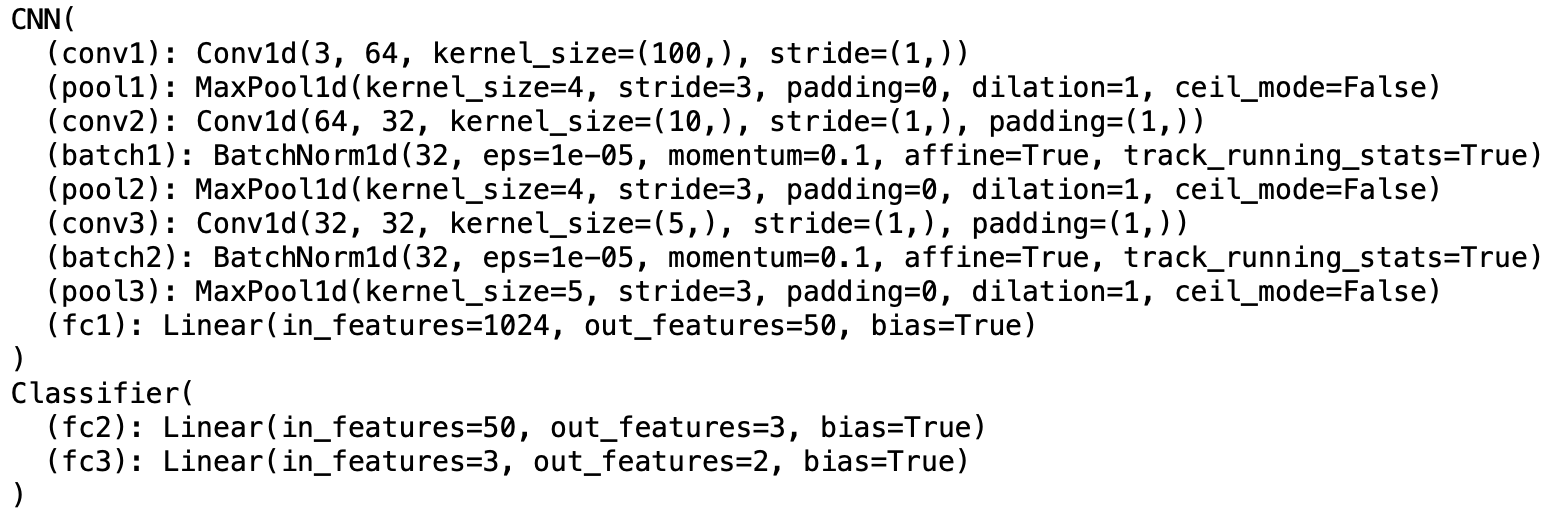
\includegraphics[width=1.1\textwidth]{model_real_data}
  \caption {MMD Model for real data} \label{fig:model_real_data}
\end{figure}
\FloatBarrier 

On the real machine dataset the three approaches regular FC + CNN MMD loss,  regular FC MMD and no MMD loss are evaluated. The accuracies on the source and target domain are visualized in fig. \ref{fig:accuracy_real_world}. In each figure three curves are presented representing different phases of the training. During the MMD Loss phase the whole model consisting of CNN and classifier are optimized with a weighted average of MMD and cross entropy loss. In the CE-Loss phase just the classifier is optimized according to a cross-entropy loss. During both phases an ADAM optimizer with a learning rate of 1e-2, beta1 of 0.9 and beta2 of 0.99 is used . In the val phase the model is evaluated. Before the training the data is split for these three phases accordingly (MMD-Loss: 60\%, CE-Loss: 20\%, Val: 20\%). Therefore all experiments follow a proper train validation split. It becomes obvious that the accuracies achieved on the validation set of the target domain were able to be increased with about 10\% by using the two MMD variations. The MMD and cross entropy loss seems to be decreased more smoothly when including CNN features into the MMD loss for the optimization of the model. Also the accuracy achieved on the target validation set achieved the regular FC + CNN MMD loss beat the one achieved with the regular FC MMD loss. Without using any MMD loss the model performance on the target domain could be increased by just around 2\%. When using the regular FC MMD loss sometimes the performance of the model breaks down  little bit. Often times this can be seen in the accuracy of the target and source domain. An example for this phenomena can be seen in fig. \ref{fig:accuracy_real_world} when looking at the accuracies of regular FC MMD (middle). In epoch ~27 the accuracy breaks down on the target and source domain. Especially during the combined training with the MMD and cross entropy loss this effect becomes especially obvious. Like mentioned in previous chapters this shows that when not including the latent features of the CNN in the MMD loss the cross entropy and MMD loss seem to work against each other, which makes the optimization less stable.

\begin{figure}[htpb]
  \centering
  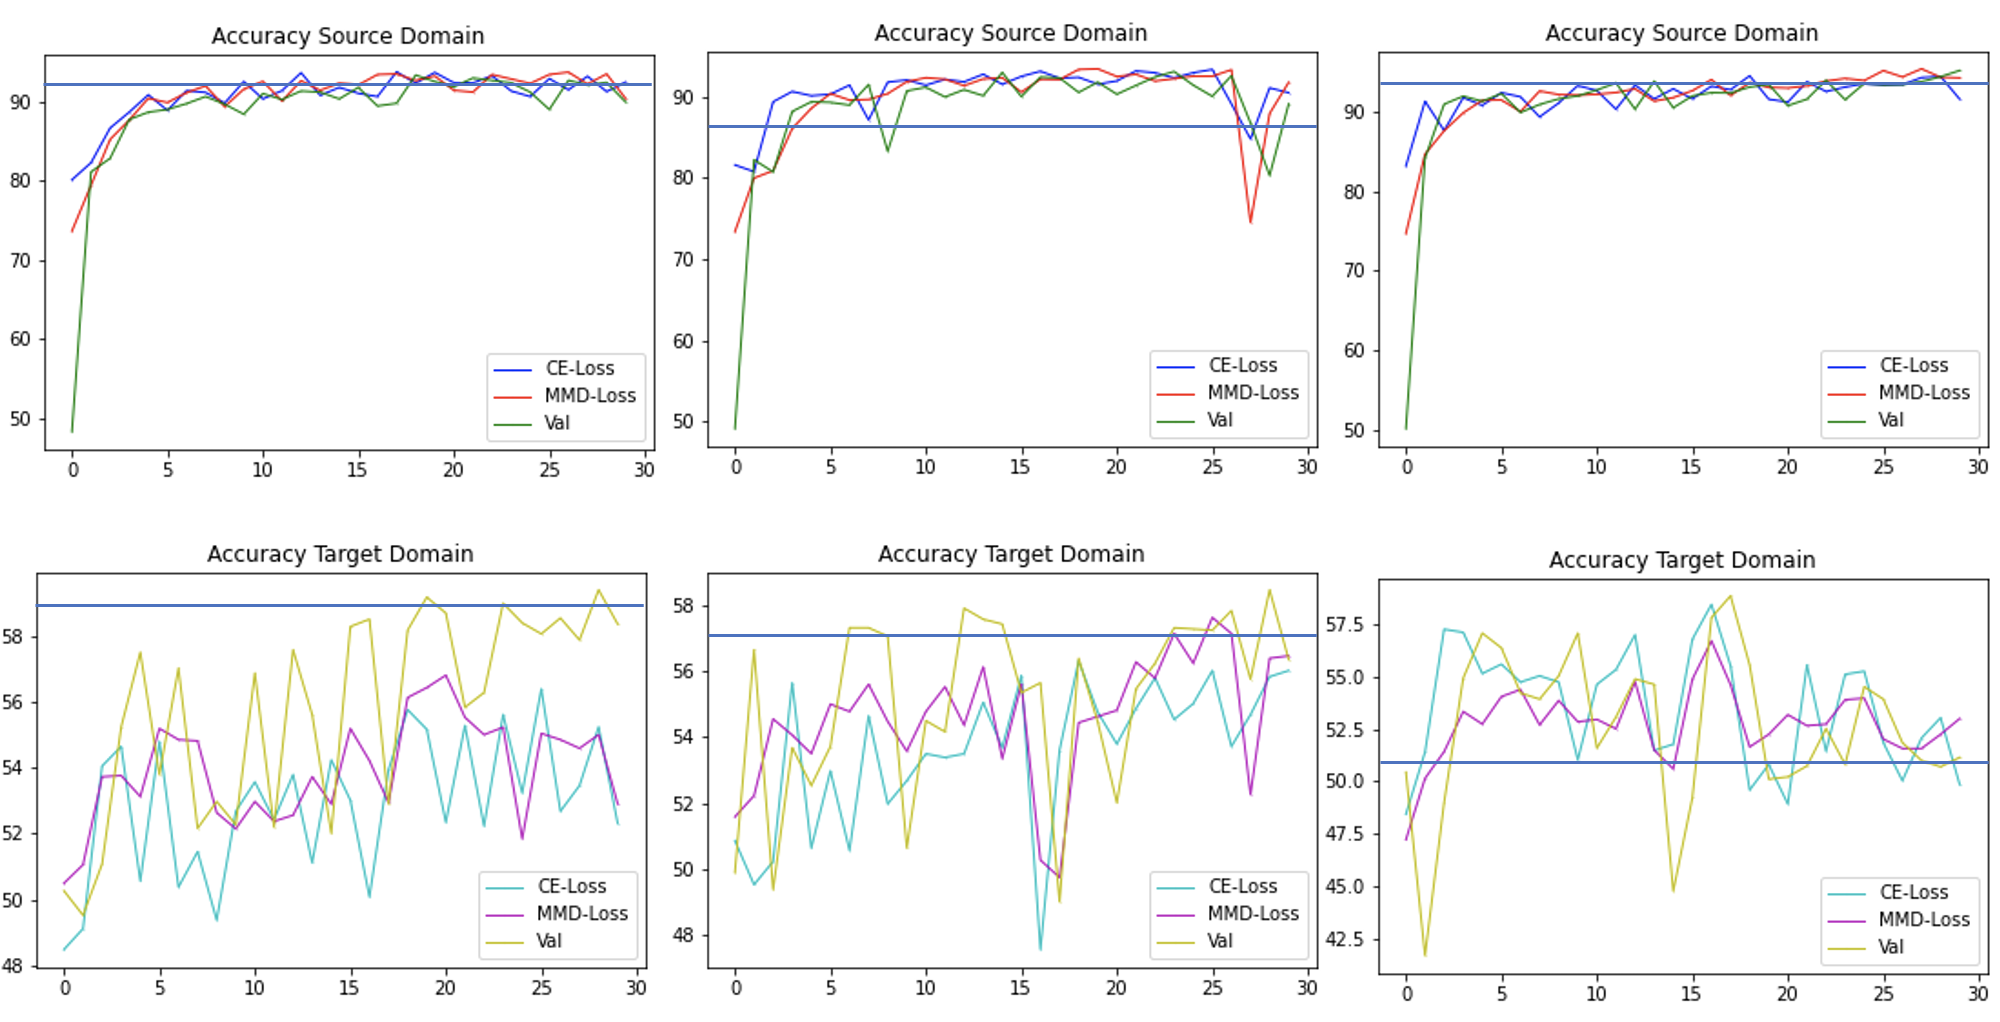
\includegraphics[width=1.1\textwidth]{accuracy_real_world}
  \caption {Accuracies for model training with Regular FC + CNN MMD loss (left), Regular FC MMD (middle) and No MMD loss (right)} \label{fig:accuracy_real_world}
\end{figure}
\FloatBarrier 

\begin{figure}[htpb]
  \centering
  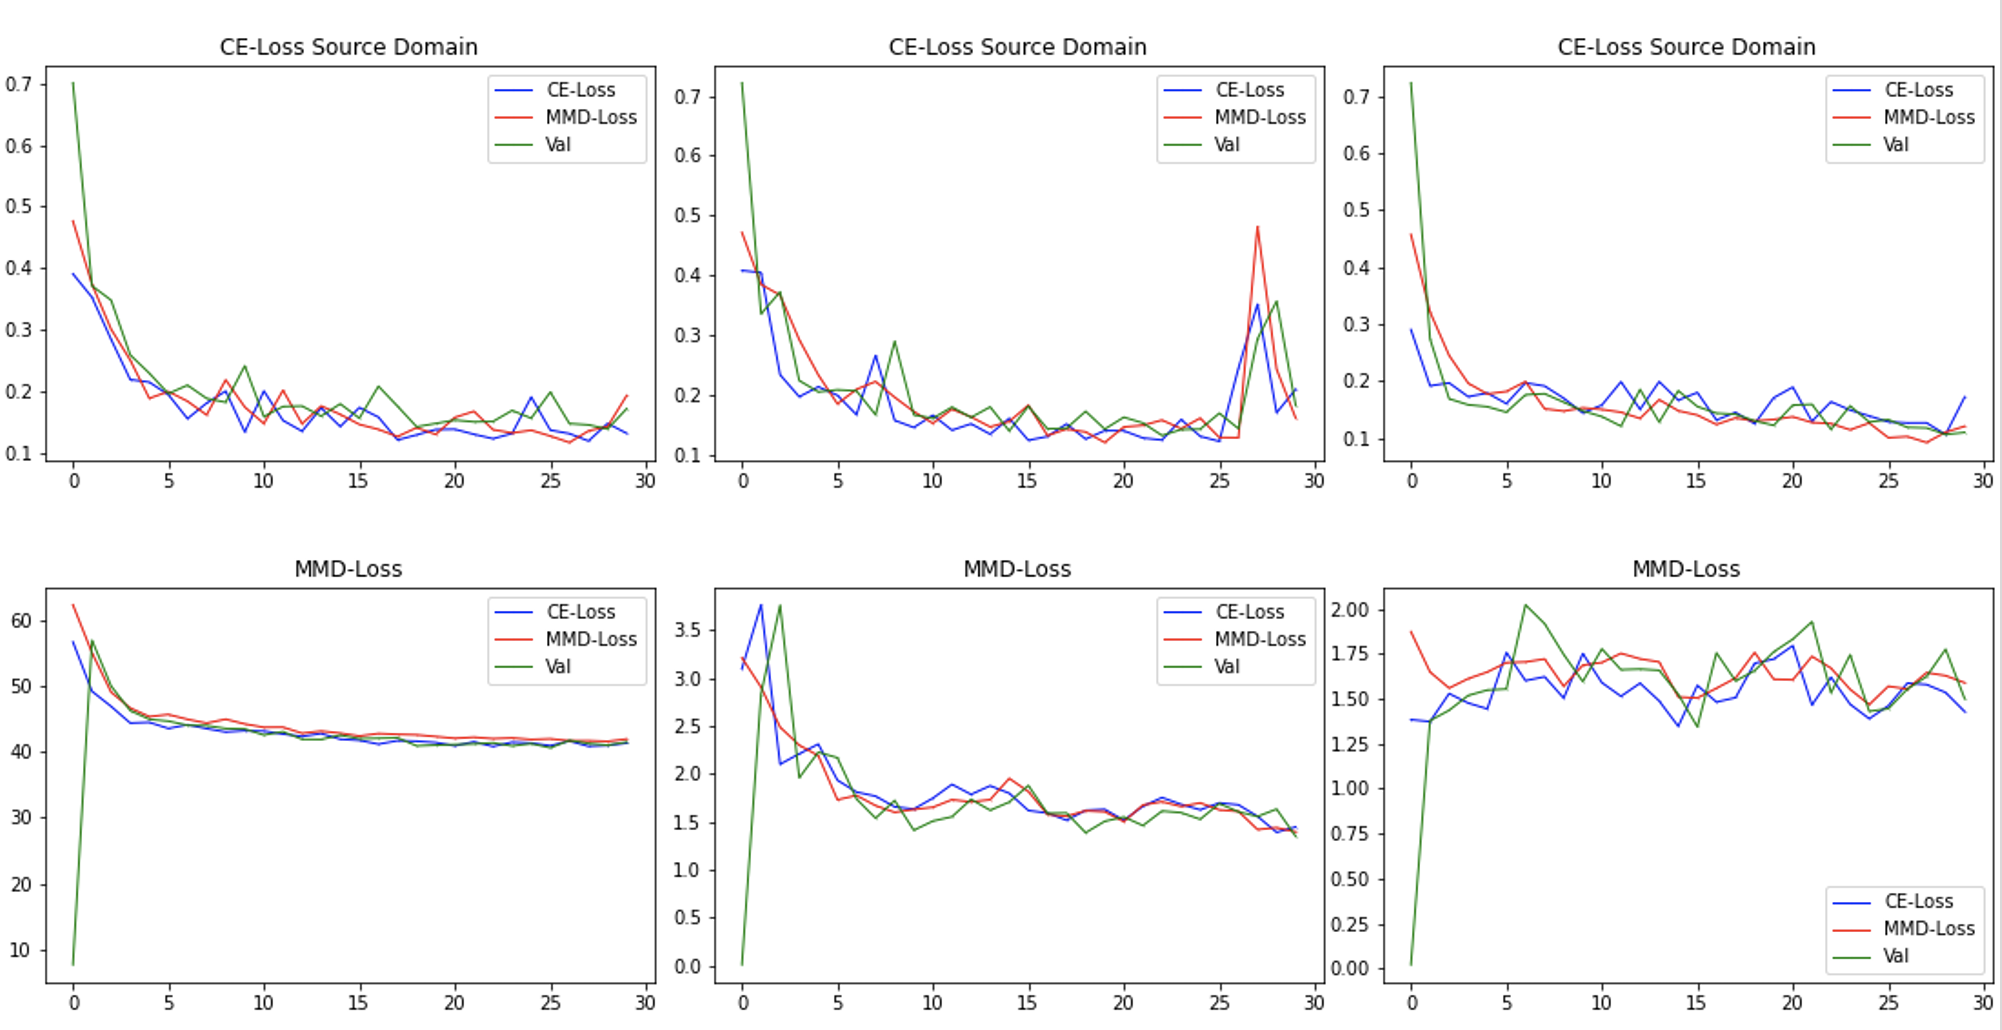
\includegraphics[width=1.1\textwidth]{loss_real_world}
  \caption {Loss for model training with Regular FC + CNN MMD loss (left), Regular FC MMD (middle) and No MMD loss} \label{fig:loss_real_world}
\end{figure}
\FloatBarrier 

In fig. the development of the source domain cross entropy MMD loss is shown. It can be seen, that the hyperparameter GAMMA was picked well, such that the MMD as well as the source cross entropy loss were able to be reduced smoothly throughout the trainings process. 


Unfortunately the MMD loss could just minimize the domain discrepancy by a little. The domain discrepancy problem couldn't be solved completely. Still the idea of the MMD loss becomes more clear in the experiments. Also the positive effect of the MMD loss for the training is obvious. For the complex multi-dimensional dataset the MMD loss is probably not sophisticated enough to detect and effectively fight the domain discrepancy.
